\documentclass[10pt]{article}
\usepackage[margin=0.85in]{geometry}
\usepackage{amsmath,amssymb,amsthm}
\usepackage{booktabs}
\usepackage{graphicx}
\usepackage{hyperref}
\usepackage{microtype}
\usepackage{xcolor}

\hypersetup{
  colorlinks=true,
  linkcolor=blue!60!black,
  citecolor=teal!70!black,
  urlcolor=blue!60!black,
  pdftitle={BitFSAI: Extreme Bit Compression for GPU Algebraic Multigrid},
  pdfauthor={Brett Bonner}
}

\newtheorem{theorem}{Theorem}

\title{\textbf{BitFSAI: Extreme Bit Compression\\
for GPU Algebraic Multigrid}}
\author{Brett Bonner\\
\small Code and Formal Proofs: \url{https://github.com/bbopen/bitfsai}}
\date{November 2026}

\begin{document}
\maketitle

\begin{abstract}
Sparse linear solvers for elliptic PDEs spend most of their GPU runtime waiting on DRAM. Four-bit weight compression relieved a similar bandwidth limit in neural networks, where small rounding errors average out across wide dense layers. Double-precision Preconditioned Conjugate Gradient (\texttt{PCG}) demands host-verified $10^{-8}$ true residuals and a symmetric positive definite (SPD) preconditioner at every iteration, so naive 4-bit rounding can inflate local eigenvalues or break convergence.

We introduce \emph{BitFSAI}, an extreme-low-bit Factorized Sparse Approximate Inverse framework for \texttt{FP64} GPU Algebraic Multigrid (AMG), combining a 4-bit zero-index GPU smoother and guarded \texttt{FP8 E5M2} coarse operators with theoretical limits extending down to 1.58-bit ternary, 1-bit sign-only, sub-bit codebooks, and zero-explicit-storage operators (with machine-checked sign-vs-ternary, cut-bound, packing, coarse-bin, and local frozen-word drift theorems). Separating positive \texttt{FP32} diagonals and row scales from signed 4-bit off-diagonals preserves $G_q^\top G_q \succ 0$ unconditionally, while a closed-form $2\times 2$ $A$-energy re-projection in \texttt{FP64} setup yields exact unit row energy for the real optimizer across both nonzero and zero off-diagonal directions and accepts the stored \texttt{FP32} scalars only when Kahan-verified patch energy satisfies $|E - 1| + 8 \epsilon_{\mathrm{mach}} \sum |t_{ab}| \le 10^{-4}$ (falling back to a verified diagonal row otherwise). Mirroring 4-bit nibbles into the matrix's symmetric CSR pattern eliminates separate factor-index arrays ($\lceil\mathrm{nnz}/2\rceil + 8n$ bytes in \texttt{bitfsai.cuh}; $\lfloor(\mathrm{nnz} + n + 1)/2\rfloor + 8n$ bytes per nonterminal level in \texttt{standalone\_amg.cu}), and scale-factored Gram application uses $4\text{ B/row}$ of ordinary smooth payload (with $8(n+1)$ bytes of library apply workspace in \texttt{bitfsai.cuh} to house fallback \texttt{double} scratch and an atomic range flag). For coarse Galerkin operators $A_c$, symmetrized row-sum diagonal repair with grounded-SDDM and normal-range $[2^{-14}, 57344]$ validation enables unscaled \texttt{FP8 E5M2} off-diagonal storage on qualifying coarse levels while falling back cleanly to \texttt{FP32} on non-M-matrix or out-of-range levels.

On an NVIDIA RTX Spark N1X across 8 SPD workloads (up to 7.08M unknowns, $10^4$ contrast, elasticity, and SuiteSparse), our 4-bit GPU implementation cuts persistent smoother factor storage by $2.75\times$--$4.45\times$ (values only) and $4.23\times$--$6.84\times$ (values plus \texttt{int32} CSR indices) versus a conventional lower-triangular \texttt{FP64} factor on the same $K \le 16$ truncated pattern, and by $2.75\times$--$6.45\times$ / $4.45\times$--$9.78\times$ versus a full-pattern lower-triangular \texttt{FSAI(1)} factor ($4.84\times$--$12.72\times$ versus mirrored \texttt{FP64} values and $1.87\times$--$3.37\times$ versus mirrored \texttt{FP16}). Integrated into NVIDIA AmgX with \texttt{FP64} outer \texttt{PCG} (fixed $\omega = 0.72$), BitFSAI passes 8/8 workloads at host \texttt{FP64} true relative residual $\le 7.86\times 10^{-9}$ with zero recoveries in timed (\texttt{step=2}) trials (while on the separate untimed \texttt{step=0} $128^3$/$192^3$ grids, all three \texttt{dFFI} smoothers trigger the $r^\top z$ guard and recover via \texttt{dDDI}). In matched \texttt{dFFI} (\texttt{FP32} inner V-cycle) precision, \texttt{INT4-spl} accelerates pure solve $1.19\times$--$4.20\times$ over matched \texttt{dFFI} \texttt{JACOBI\_L1} on 6/8 workloads (near-parity $1.05\times$ on $128^3$, $0.90\times$ on \texttt{tet48}), wins paired \texttt{resetup + solve} on the two stiffest structural matrices ($2.65\times$ on \texttt{bcsstk14}, $2.68\times$ on \texttt{bcsstk15}; diagonal \texttt{JACOBI\_L1} wins paired time on the other 6 workloads at $0.37\times$--$0.86\times$, reflecting BitFSAI's resetup path including CSR validation, per-row Cholesky, and patch-energy checks), and runs at $1.00\times$--$1.12\times$ solve ($0.99\times$--$1.19\times$ paired) versus \texttt{dFFI} \texttt{BitFSAI FP16}; combining the \texttt{dDDI}-to-\texttt{dFFI} inner-cycle precision change with \texttt{INT4-spl} accelerates pure solve $1.07\times$--$4.38\times$ over stock \texttt{dDDI} \texttt{JACOBI\_L1} across all 8 workloads. In our standalone CUDA-Graph AMG engine on the $192^3$ $10^4$-contrast problem, combining SDDM- and normal-range-guarded \texttt{FP8 E5M2} coarse operators ($1.86\times$ smaller coarse apply-value buffers, $400.6\text{ MiB}$ to $215.8\text{ MiB}$) with sparse-depth polynomial boosting cuts iterations from 28 to 13 and speeds up GPU solve time $1.53\times$ ($1511.1\text{ ms}$ to $990.4\text{ ms}$; paired $1.03\times$, parity within overlapping 3-trial ranges, with \texttt{build\_fp8\_coarse} performing D2H transfer and host-side connected-component grounding checks during resetup; \texttt{poly4@2} with \texttt{FP32} $A_c$ reaches $1.48\times$ solve and $1.36\times$ paired from $1833.3\text{ ms}$ to $1347.9\text{ ms}$) versus \texttt{INT4-spl} + \texttt{FP32} $A_c$, while reducing stored smoother-factor plus nonterminal coarse apply-value buffers $1.46\times$ ($589.8\text{ MiB}$ to $405.0\text{ MiB}$, saving $184.82\text{ MiB}$) and combined active smoother + coarse-$A_c$ storage $3.51\times$ versus conventional lower-triangular \texttt{FP64} (values + indices) + \texttt{FP32} $A_c$ ($3.90\times$ versus mirrored \texttt{FP64} + \texttt{FP32} $A_c$).

To establish asymptotic guarantees and fundamental bit-compression limits, we prove a monotone multilevel effectiveness recurrence with both directions of the periodic work-convergence frontier $\beta^2 < p$, dimension-, depth-, and contrast-independent spectral condition bounds $\kappa_2(A_0^{1/2} B_0 A_0^{1/2}) \le 17$ (at $t = 2560/1307$) and $\le 9$ (at $t = 30375/15853$) in $O(m+n)$ per-cycle work for certified grounded SDDM hierarchies, an $O((m+n)W^2)$ normalized-kernel finite-precision bit-complexity bound, and sharp sub-4-bit limits: an exact Schur-pivot criterion $D/\sigma \le (K-1)^2/(4K)$ and arbitrary-$n$ Global Kaporin Product Identity, a 3-vertex grounded-SDDM separation proving 1-bit sign-only diverges ($\kappa \sim 2/t$) where 1.58-bit ternary converges ($\kappa \to 1$), a contrast-independent $r+1$ ternary threshold-cut bound for arbitrary $r$-predecessor grounded SDDM patches (matching the $(r+1)/2$ path lower bound in order), projective SPD covering limits down to sub-bit and 0-bit physics-reconstructed operators, and $h/l$ and Kantorovich quadratic $1 + (h-l)^2/(4hl)$ local frozen-word drift bounds for changing nonlinear tangent operators. All 65 algebraic, Galerkin, operator-effectiveness, scalar-recurrence, bit-limit, and drift theorems are machine-checked in Lean~4 + Mathlib (zero \texttt{sorry}, standard axioms only), complemented by 142 Z3 SMT UNSAT obligations (+ 10 SAT controls, spanning exact-real core/multilevel/bit-limit bounds and exhaustive bit-level \texttt{BitVec} \texttt{INT4}/\texttt{FP4}/\texttt{FP8} encoding proofs), host C++17 checks, exact-rational/finite-grid audits across 14 grounded SDDM roots, 2 edge-pruned hierarchies, and 63 normalized solves, and clean 4/4 \texttt{compute-sanitizer} verification (\texttt{memcheck}, \texttt{racecheck}, \texttt{initcheck}, \texttt{synccheck}).
\end{abstract}

\section{Introduction}\label{sec:intro}
Discretizing heat diffusion, linear elasticity, or subsurface flow on a 3D mesh yields a large sparse SPD linear system
\[
  A x = b, \qquad A \in \mathbb{R}^{n \times n}, \qquad A = A^\top \succ 0.
\]
Each row couples an unknown to 7 to 75 nearby nodes, while $n$ reaches millions. Production solvers pair Preconditioned Conjugate Gradient (\texttt{PCG})~\cite{hestenes1952cg} with Algebraic Multigrid (\texttt{AMG})~\cite{brandt1986algebraic,ruge1987algebraic,trottenberg2001multigrid}. A smoother damps local high-frequency error on each level, coarse Galerkin operators $A_c = P^\top A P$ resolve global modes at reduced size, and an outer \texttt{FP64} \texttt{PCG} loop monitors $r = b - A x$ until $\|b - A x\|_2 / \|b\|_2 \le 10^{-8}$.

On a modern GPU, reading one \texttt{FP64} nonzero and its \texttt{int32} column index moves 12 bytes to perform two floating-point operations---an arithmetic intensity below $0.17\text{ FLOP/byte}$, two orders of magnitude below hardware compute balance. Existing GPU smoothers pay for that gap in different ways. Diagonal smoothers such as \texttt{l1-Jacobi} read minimal extra memory yet require hundreds of iterations on anisotropic, high-contrast, or elasticity problems. Incomplete Cholesky (\texttt{IC(0)})~\cite{meijerink1977ic,vacek2025mixed} relies on sequential triangular solves (\texttt{SpTrSV}) that underutilize GPU warps and amplify quantization noise along elimination chains. Conventional lower-triangular Factorized Sparse Approximate Inverse (\texttt{FP64 FSAI})~\cite{kolotilina1993fsai,janna2015fsaipack} runs completely in parallel and roughly halves iteration counts, yet stores $8.0\text{ B/nnz}_L$ of factor weights alongside $4$ to $8\text{ B/nnz}_L$ of separate CSR indices (where $\mathrm{nnz}_L = (\mathrm{nnz}(A) + n)/2$), whereas a mirrored full-CSR \texttt{FP64} factor stores $8.0\text{ B/nnz}(A)$.

Four-bit and sub-8-bit weight formats (\texttt{INT4}, \texttt{NF4}, and \texttt{FP8}) cut memory traffic dramatically in neural networks~\cite{dettmers2022llmint8,micikevicius2022fp8,frantar2023gptq,dettmers2023qlora}, where rounding errors average across wide dense layers. Inside \texttt{FP64} \texttt{PCG} targeting host-verified $10^{-8}$ residuals, the preconditioner $M$ must remain symmetric positive definite ($r^\top M r > 0$) and spectrally bounded on every iteration: zeroing a single diagonal entry or inflating one local eigenvalue triggers the \texttt{PCG} curvature guard ($r^\top z \le 0$) and aborts or restarts the solve.

This paper develops \emph{BitFSAI} across both GPU systems and multilevel theory:
\begin{enumerate}
  \item \emph{Row-level stability and zero-index GPU architecture (Sections~\ref{sec:principles}--\ref{sec:gpu_alg}):} We establish four algebraic principles---Gram-SPD invariance, diagonal-split necessity, closed-form $2\times 2$ $A$-energy re-projection (including its zero-direction fallback), and scale-factored Gram application---together with symmetrized row-sum diagonal repair for unscaled \texttt{FP8 E5M2} coarse operators, yielding a 4-bit smoother with zero extra CSR indices ($0.5\text{ B/nnz}(A) + 8\text{ B/row}$) and a CUDA-Graph-capturable multilevel preconditioner.
  \item \emph{Live Blackwell GPU evaluation (Section~\ref{sec:eval}):} Across 8 SPD workloads on an NVIDIA RTX Spark N1X, we evaluate our standalone CUDA AMG engine (\texttt{reference/standalone\_amg.cu}), a four-engine comparison against NVIDIA AmgX~\cite{naumov2015amgx} (in both matched \texttt{dDDI} and matched \texttt{dFFI} precision), LLNL \texttt{hypre}~\cite{falgout2002hypre}, and Ginkgo~\texttt{develop} (\texttt{2.0.0-dev})~\cite{anzt2022ginkgo}, and GPU silicon realizations of SDDM- and normal-range-guarded \texttt{FP8 E5M2} coarse operators with sparse-depth polynomial boosting under an explicit per-engine timing and host \texttt{FP64} residual verification protocol ($\le 10^{-8}$).
  \item \emph{Asymptotic multilevel guarantees and extreme-low-bit limits (Section~\ref{sec:theory}):} We prove a three-pass certified damping guard with an arbitrary-dimensional Galerkin Loewner sandwich (and its $2\times 2$ overdamping obstruction), a monotone multilevel effectiveness recurrence (single-level operator step mechanized directly in $A$-inner-product form) with both directions of the periodic work-convergence product-inequality frontier $\beta^2 < p$, dimension- and contrast-independent root condition bounds $\kappa_2(A_0^{1/2} B_0 A_0^{1/2}) \le 17$ and $\kappa_2(A_0^{1/2} B_0 A_0^{1/2}) \le 9$ in $O(m+n)$ per-cycle work for certified grounded SDDM hierarchies, a power-of-two-normalized $O((m+n)W^2)$ finite-precision bit-complexity bound alongside state/output lower bounds, and sharp sub-4-bit precision limits (Theorem~9: exact Schur-pivot criterion $D/\sigma$, arbitrary-$n$ Global Kaporin Product Identity, 1-bit sign vs.\ 1.58-bit ternary separation, contrast-independent $r+1$ grounded-SDDM ternary cut bound, sub-bit/0-bit information-theoretic regimes, and frozen-word drift bounds for changing nonlinear tangent operators). All 65 core, multilevel, bit-limit, and drift theorems are machine-checked in Lean~4 + Mathlib~\cite{demoura2021lean4,mathlib2020} alongside 142 Z3 SMT obligations~\cite{demoura2008z3} (109 core/multilevel exact-real + 12 exhaustive \texttt{BitVec} encoding + 21 bit-limit/drift exact-real obligations). While our theoretical bounds extend down to ternary, sub-bit, and zero-storage operators, the GPU implementation and empirical evaluation in this paper remain focused on 4-bit zero-index smoothers and guarded \texttt{FP8 E5M2} coarse operators.
\end{enumerate}

\section{Background and Related Work}\label{sec:background}
Kolotilina and Yeremin~\cite{kolotilina1993fsai} introduced Factorized Sparse Approximate Inverse (\texttt{FSAI}), minimizing $\|I - G L\|_F^2$ (with $A = L L^\top$) over lower-triangular matrices $G$ with a prescribed sparsity pattern. Kaporin~\cite{kaporin1994new} showed that the row-wise optimal factor also minimizes the Kaporin condition number of $G A G^\top$. Because every row solves an independent small SPD system over its lower-triangle neighbors, setup and application ($t = G r$, $z = G^\top t$) are fully parallel. Adaptive CPU and GPU implementations appear in \texttt{FSAIPACK}~\cite{janna2015fsaipack}, \texttt{Chronos}~\cite{isotton2021chronos}, LLNL \texttt{hypre}~\cite{falgout2002hypre,yang2002boomeramg}, and extended-pattern GPU \texttt{FSAI}~\cite{laut2024gfsai}, all storing lower-triangular factor values in \texttt{FP64} or \texttt{FP32} with separate factor index arrays.

Mixed-precision sparse preconditioners in Ginkgo~\cite{anzt2022ginkgo} lowered storage precision to 16 bits. Flegar et al.~\cite{flegar2021adaptive} stored adaptive block-Jacobi inverses down to \texttt{FP16} and \texttt{INT16}. G\"obel et al.~\cite{gobel2021mixed} decoupled storage and compute precision for Incomplete Sparse Approximate Inverses (\texttt{ISAI}) down to \texttt{FP16} while retaining separate index arrays. Tsai, Beams, and Anzt~\cite{tsai2023three} studied three-precision (\texttt{FP64}/\texttt{FP32}/\texttt{FP16}) GPU AMG in Ginkgo, and Vacek et al.~\cite{vacek2025mixed} analyzed mixed-precision \texttt{IC}-smoothed multigrid building on Meijerink and van der Vorst's \texttt{IC(0)} factorization~\cite{meijerink1977ic}. Production GPU AMG libraries include NVIDIA AmgX~\cite{naumov2015amgx} (classical \texttt{PMIS-D2} and aggregation~\cite{notay2010agmg}), LLNL \texttt{hypre} \texttt{BoomerAMG}~\cite{falgout2002hypre,yang2002boomeramg} (\texttt{PMIS} and \texttt{ext+i} with \texttt{l1-Jacobi} or GPU \texttt{FSAI}), Ginkgo~\cite{anzt2022ginkgo} (\texttt{PGM} multigrid with \texttt{SpdIsai}), and device-resident blocked GPU AMG with symbolic \texttt{RAP} reuse in PETSc~\cite{adams2026blocked,adams2026galerkin}.

On the multilevel theory side, algebraic multilevel iteration (\texttt{AMLI})~\cite{axelsson1989amli}, recursive Krylov \texttt{K}-cycles~\cite{notay2008kcycle}, and guaranteed-rate \texttt{AMLI}~\cite{napov2012amli} establish polynomial scheduling for level-independent convergence; approximate Schur complements and linear-size spectral sparsification~\cite{durfee2017schur,lee2015sparsification} yield near-linear graph-Laplacian coarsening; and McCormick, Benzaken, and Tamstorf~\cite{mccormick2021mixed,mccormick2023rounding} analyze rounding error in mixed-precision multigrid. Prior GPU sparse smoothers stop at 16-bit storage. BitFSAI reaches 4-bit mirrored factor weights ($0.5\text{ B/nnz}(A) + 8\text{ B/row}$) with zero duplicate CSR indices, pairs post-quantization $2\times 2$ $A$-energy re-projection with SDDM- and normal-range-guarded row-sum-repaired \texttt{FP8 E5M2} coarse operators on live GPU silicon, and provides machine-checked proofs spanning both row stability and asymptotic multilevel convergence.

\section{Smoother Design Principles and Coarse-Grid Precision}\label{sec:principles}
We first establish the four algebraic rules that make 4-bit factorized smoothing numerically sound and bandwidth-efficient, followed by the precision floor for coarse Galerkin operators. All 21 smoother and row-sum repair theorems in this section are machine-checked in Lean~4 + Mathlib (\texttt{proofs/lean/Bitfsai/Core.lean}, zero \texttt{sorry}, standard axioms only; audit in Section~\ref{sec:audit}).

\subsection{Gram-SPD Invariance, Diagonal Splitting, and Row Re-Projection}
On a 3D $20^3$ anisotropic ($10^{-3}, 1, 10^{-2}$), $10^4$-contrast diffusion problem solved by a \emph{two-grid cycle} with an exact \texttt{LU} coarse solve (\texttt{benchmarks/quant\_cliff\_and\_coarse\_floor.py}), 25 power iterations heuristically estimate $\lambda_{\max}(M_q A)$ at $1.69$ for \texttt{FP64} \texttt{IC(0)} versus $12.28$ at diagonal-inclusive \texttt{INT3} ($8.63$ at \texttt{INT2}). Consequently, undamped \texttt{IC(0)} ($\omega = 1$) suffers non-SPD two-grid breakdown at \texttt{INT3} and \texttt{INT2}, and even heuristic spectral damping ($\omega = \min(1, 1.4/\hat{\lambda}_{\max})$) degrades \texttt{IC(0)} from $10$ iterations (\texttt{FP64}) to $16$ (\texttt{INT3}) and $25$ (\texttt{INT2}) (Figure~\ref{fig:principles}a; note that \texttt{IC(0)} is tested with diagonal-inclusive quantization without a split-encoded \texttt{IC(0)} control). By contrast, an explicit factorized smoother evaluates $M_q = G_q^\top G_q$ directly without triangular inversion, keeping its quadratic form a sum of squares $x^\top(G_q^\top G_q)x = \|G_q x\|_2^2$, holding $\hat{\lambda}_{\max}(M_q A)$ near $1.70$, and converging in $14$ \texttt{PCG} iterations at fixed $\omega = 0.72$ down to \texttt{INT2}. On this structured 7-point grid where diagonal-to-off-diagonal ratios are bounded, the diagonal-inclusive \texttt{INT4} \texttt{BitFSAI} control (\texttt{INT4inc}) likewise stays stable ($\hat{\lambda}_{\max} = 1.67$, $13$ iterations); as Theorem~2 proves below, diagonal splitting becomes essential once row diagonals dominate off-diagonals on ill-conditioned or stiff matrices.

\begin{theorem}[Gram-SPD Invariance, arbitrary $n \in \mathbb{N}$]
For any $n \in \mathbb{N}$ and any lower-triangular $G \in \mathbb{R}^{n \times n}$ with strictly positive diagonal entries ($\forall i,\; G_{ii} > 0$), $G$ is injective and $M = G^\top G$ is symmetric positive definite (\texttt{Matrix.PosDef}), regardless of how the strictly lower off-diagonal entries are quantized. Conversely, if quantization rounds any diagonal entry $G_{kk} = 0$, then $\det(G^\top G) = 0$ and $G^\top G$ fails to be positive definite (\texttt{lowerTriangular\_posDiag\_injective}, \texttt{gram\_posDef\_of\_lowerTriangular\_posDiag}, \texttt{diagonal\_split\_preserves\_posDef}, \texttt{lowerTriangular\_zero\_diag\_not\_posDef}).
\end{theorem}

Protecting the diagonal is required for conditioning as well as invertibility. Analogous to outlier channels in transformer quantization~\cite{dettmers2022llmint8,dettmers2023qlora}, an \texttt{FSAI} row diagonal $g_{ii}$ can exceed its off-diagonal couplings by orders of magnitude. When a single row scale spans both $g_{ii}$ and the off-diagonals (diagonal-inclusive \texttt{INT4}), small off-diagonal couplings round straight to zero.

\begin{theorem}[Spectral Distortion and $2\times 2$ Diagonal-Split Necessity]
Let $A \in \mathbb{R}^{n \times n}$ be SPD, $G \in \mathbb{R}^{n \times n}$ be nonsingular, and $G_q = (I + E)G$ with $\|E u\|_2 \le \eta \|u\|_2$ for all $u \in \mathbb{R}^n$ and $0 \le \eta < 1$. For every dimension $n$ and all nonzero $x, y \in \mathbb{R}^n$, both the vector-norm sandwich and the pointwise generalized Rayleigh-quotient distortion bound hold:
\[
  (1 - \eta)^2 \|u\|_2^2 \le \|u + E u\|_2^2 \le (1 + \eta)^2 \|u\|_2^2, \qquad
  \frac{\|G_q x\|_2^2 / (x^\top A x)}{\|G_q y\|_2^2 / (y^\top A y)} \le \left(\frac{1+\eta}{1-\eta}\right)^2 \frac{\|G x\|_2^2 / (x^\top A x)}{\|G y\|_2^2 / (y^\top A y)}.
\]
Lean mechanizes this pointwise two-vector inequality for every SPD denominator (\texttt{conditional\_spectral\_distortion\_bound}, \texttt{rayleigh\_condition\_distortion\_bound}); substituting $A \mapsto A^{-1}$ and taking the supremum over $x \neq 0$ and infimum over $y \neq 0$ yields the extremal condition-number corollary $\kappa_2(G_q A G_q^\top)/\kappa_2(G A G^\top) \le ((1+\eta)/(1-\eta))^2$ (strictly below $2.06$ at the illustrative perturbation budget $\eta = 5/28$, equal to $2.5$ times the symmetric \texttt{INT4} half-step $1/14$; \texttt{eta\_five\_over\_28\_bound}). The distortion factor $((1+\eta)/(1-\eta))^2$ is attained for every $\eta \in [0, 1)$ (e.g., $E = \operatorname{diag}(\eta, -\eta)$ on $G = I, A = I$), while at $\eta = 1$ singularity ($I + E$ non-invertible) makes the ratio unbounded. Separately, to expose diagonal-inclusive \texttt{INT4} collapse on stiff rows, consider the SPD matrix
\[
  A_{\mathrm{ex}} = \begin{bmatrix}1 & 1/25\\ 1/25 & 17/10000\end{bmatrix} \succ 0, \qquad
  G_{\mathrm{ex}} = \begin{bmatrix}1 & 0\\ -4 & 100\end{bmatrix}, \qquad
  G_{\mathrm{ex}} A_{\mathrm{ex}} G_{\mathrm{ex}}^\top = I.
\]
Diagonal-inclusive symmetric \texttt{INT4} (step $100/7$) rounds $-4$ to $0$ because $|-4/(100/7)| < 1/2$, inflating the preconditioned condition number from $\kappa_2 = 1$ above $321$ ($\operatorname{tr} = 18$, $\det = 1$). Keeping $g_{ii}$ in \texttt{FP32} and scaling only the off-diagonals (diagonal-split \texttt{INT4-spl}) encodes $-4$ with code $-7$ and scale $4/7$, recovering $G_{\mathrm{ex}} A_{\mathrm{ex}} G_{\mathrm{ex}}^\top = I$ identically (\texttt{split\_int4\_recovers\_exact\_factor}, \texttt{counterexample\_2x2\_kappa\_gt\_321}).
\end{theorem}

Even when $M = G_q^\top G_q \succ 0$, the condition $\omega \lambda_{\max}(M A) < 2$ is necessary and sufficient for strict positivity of the \emph{symmetrized smoother} $2M - \omega M A M \succ 0$, and sufficient for strict positivity of the full V-cycle whenever the coarse correction is PSD. On $A_{\mathrm{ex}}$, diagonal-inclusive \texttt{INT4} produces $M \succ 0$ yet makes $2M - 0.65 M A_{\mathrm{ex}} M$ indefinite (\texttt{gram\_spd\_not\_sufficient\_for\_fixed\_damping}). On stiff structural matrices (\texttt{bcsstk14}, \texttt{bcsstk15} in Section~\ref{sec:four_engine}), disabling row re-projection in \texttt{dFFI} triggers outer \texttt{PCG} curvature-guard (\texttt{rz}) failures (recording non-positive $r^\top z$ at the outer cycle level without isolating a single level or component), which re-projection in the $A$-norm eliminates.

\begin{theorem}[Optimal $2\times 2$ $A$-Energy Re-Projection and Zero-Direction Fallback]
Let $w_{\mathrm{off}}$ be the decoded 4-bit off-diagonal vector for row $i$ with patch Cholesky factor $A_{\mathrm{patch}} = L L^\top$, Gram scalars $c_{11} = \|L^\top w_{\mathrm{off}}\|_2^2 \ge 0$, $c_{12} = (L^\top w_{\mathrm{off}})^\top(L^\top e_m)$, and $c_{22} = A_{ii} > 0$:
\begin{enumerate}
  \item \emph{Nonzero off-diagonal branch ($c_{11} > 0$, $\Delta = c_{11}c_{22} - c_{12}^2 > 0$):} setting
  \[
    g_{ii}^* = \sqrt{\frac{c_{11}}{\Delta}} > 0, \qquad s_i^* = -\frac{c_{12}}{\sqrt{c_{11}\Delta}}
  \]
  guarantees $g_{ii}^* > 0$ (preserving Theorem~1), exact unit $A$-energy $(G_q A G_q^\top)_{ii} = 1$, and global optimality of Kaporin's local ratio $(g^\top A_{\mathrm{patch}} g)/g_{ii}^2$ over all $(s,g) \in \mathbb{R}\times\mathbb{R}_{>0}$ (\texttt{optimal\_2x2\_reprojection\_properties}).
  \item \emph{Zero off-diagonal fallback branch ($c_{11} = c_{12} = 0$, $c_{22} > 0$):} when all quantized off-diagonals vanish, setting $s_i^* = 0$ and $g_{ii}^* = 1/\sqrt{c_{22}}$ likewise guarantees $g_{ii}^* > 0$, exact unit $A$-energy $(g_{ii}^*)^2 c_{22} = 1$, and global Kaporin optimality (\texttt{zero\_offdiag\_reprojection\_fallback}). On $A_{\mathrm{ex}}$ after inclusive \texttt{INT4} zeroes the off-diagonal ($c_{11} = 0$), this diagonal fallback yields $G_{\mathrm{ren}} = \operatorname{diag}(1, 100/\sqrt{17})$ and restores \texttt{Matrix.PosDef} of $2M - 0.72 M A_{\mathrm{ex}} M$ (\texttt{renormalized\_2x2\_counterexample\_posDef}).
\end{enumerate}
\end{theorem}

To avoid catastrophic cancellation when $c_{12}^2 \approx c_{11}c_{22}$, our CUDA implementation (\texttt{reference/row\_projection.hpp}) computes the component of $v = L^\top e_m$ orthogonal to $u = L^\top \tilde{q}$ in \texttt{FP64}, casts $(g_{ii}^*, s_i^*)$ to \texttt{FP32}, re-evaluates the stored row's patch energy against the CSR entries with Kahan summation, and accepts only if $|E - 1| + 8 \epsilon_{\mathrm{mach}} \sum |t_{ab}| \le 10^{-4}$ (otherwise replacing the row with the verified diagonal fallback $g_{ii} = A_{ii}^{-1/2}$).

\subsection{Zero-Index CSR Sharing and Scale-Factored Application}
Compressing factor weights to 4 bits ($0.5\text{ B/nnz}(A)$) causes an \emph{index-bandwidth inversion} if separate \texttt{int32} column indices are stored and read: streaming separate factor indices in Pass~1 and Pass~2 moves $8.0\text{ B/nnz}_L$, dominating weight traffic. Because \texttt{FSAI(1)} uses $A$'s lower-triangle sparsity pattern, setup mirrors each quantized 4-bit off-diagonal nibble into both the lower slot $k_{\mathrm{low}}$ in row $i$ and the symmetric upper slot $k_{\mathrm{up}}$ in row $j$, allocating $0\text{ B}$ of separate factor indices. Both apply passes stream $A$'s existing \texttt{row\_offsets} and \texttt{col\_indices} directly.

\begin{theorem}[Scale-Factored Gram Identity, arbitrary $n \in \mathbb{N}$]
For any row-scale vector $s \in \mathbb{R}^n$ and unscaled factor $\tilde{G} \in \mathbb{R}^{n \times n}$, $G = \operatorname{diag}(s)\tilde{G}$ satisfies
\[
  (G^\top G) x = \tilde{G}^\top \bigl(\operatorname{diag}(s^2)(\tilde{G} x)\bigr) \qquad \forall x \in \mathbb{R}^n.
\]
In the ordinary \texttt{FP32} path, Pass~1 writes $y_i = s_i t_i$ ($4\text{ B/row}$ smooth scratch), eliminating all random \texttt{s[c]} global-memory gathers in Pass~2 (\texttt{scale\_factored\_gram\_identity}). When extreme matrix scales risk \texttt{FP32} underflow or overflow in $s_i t_i$, the apply path disables factoring and restores source scales $s_{c_k}$ in Pass~2 with \texttt{double} accumulation.
\end{theorem}

\subsection{Precision Tiering and Row-Sum-Repaired \texttt{FP8 E5M2} Coarse Operators}
Unlike fine-level smoothers, coarse Galerkin operators $A_c = P^\top A P$ under $10^4$ coefficient contrast require dynamic range across 8 orders of magnitude and constant-mode preservation. Symmetrizing $Q = Q^\top$ and replacing quantized diagonals with $\tilde{A}_{ii} = A_{ii} + \sum_{k \neq i}(A_{ik} - Q_{ik})$ guarantees $\tilde{A}\mathbf{1} = A\mathbf{1}$ for every dimension $n$, and preserves M-matrix diagonal dominance whenever original row sums are nonnegative and quantized off-diagonals are nonpositive (\texttt{rowSum\_repair\_preserves\_ones}, \texttt{rowSum\_repair\_diag\_dom}). On the 3D $20^3$ $10^4$-contrast test (Figure~\ref{fig:principles}b, Table~\ref{tab:coarse}), naive \texttt{FP16} and \texttt{FP8} break down in 1--3 iterations, \texttt{INT8} with row-sum repair stalls at the 400-iteration limit (whereas naive per-row-scaled \texttt{INT8} converges in 155 iterations), and unscaled \texttt{FP8 E5M2} (5 exponent bits, normal range $[2^{-14}, 57344]$ enforced strictly against saturation and subnormals) with row-sum repair matches \texttt{FP64} in $14$ iterations with an \texttt{FP64} diagonal ($4.06\times 10^{-9}$ vs.\ $2.55\times 10^{-9}$) and converges in $15$ iterations ($6.55\times 10^{-9}$) with an upward-guarded \texttt{FP32} diagonal---requiring zero per-row scale metadata (unlike per-row-scaled \texttt{FP16}, \texttt{INT8}, and \texttt{FP8 E4M3}).

\begin{figure}[t]
  \centering
  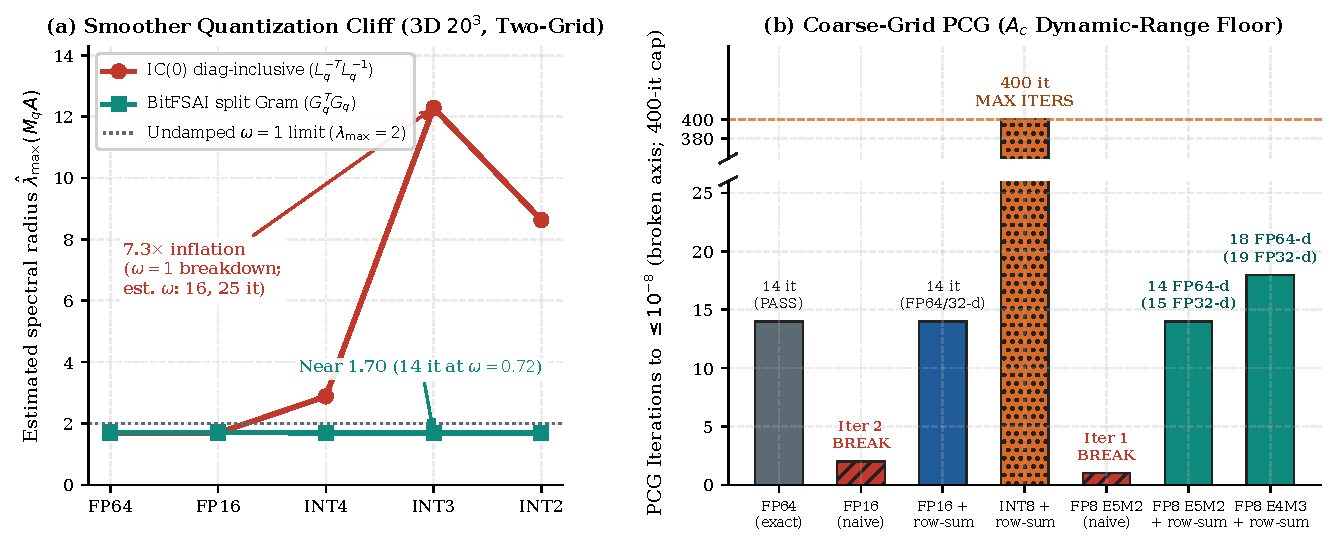
\includegraphics[width=\textwidth]{figures/fig1_quant_cliff_and_coarse.pdf}
  \caption{Smoother and coarse-grid precision limits on a 3D $20^3$ anisotropic ($10^{-3}, 1, 10^{-2}$), $10^4$-contrast SPD PDE ($N = 8{,}000$, $N_c = 4{,}000$), plotted directly from \texttt{benchmarks/results/cpu\_precision\_sweep.csv}. (a)~Two-grid cycle with exact \texttt{LU} coarse solve: diagonal-inclusive \texttt{IC(0)} exhibits a $7.3\times$ spectral-radius cliff at \texttt{INT3} causing $\omega = 1$ breakdown ($16$ / $25$ iterations under heuristic damping), while split, reprojected BitFSAI stays near $1.70$ ($14$ iterations at $\omega = 0.72$) down to \texttt{INT2} (and the \texttt{INT4inc} control stays at $\hat{\lambda}_{\max} = 1.67$, $13$ iterations on this grid). (b)~Coarse-grid \texttt{PCG} iterations on a broken linear y-axis ($400$-iteration cap): plotted naive \texttt{FP16}/\texttt{FP8 E5M2} break down in 1--2 iterations (\texttt{FP8 E4M3} naive breaks down at 3 iterations in Table~\ref{tab:coarse}) and \texttt{INT8 + row-sum} stalls at $400$ iterations, whereas unscaled \texttt{FP8 E5M2} + row-sum converges in $14$ iterations with \texttt{FP64} diagonal ($15$ with guarded \texttt{FP32} diagonal).}
  \label{fig:principles}
\end{figure}

\begin{table}[t]
\centering\small
\begin{tabular}{@{}lrrll@{}}
\toprule
Coarse $A_c$ Format & Off-Diag Bits & PCG Iters & True Rel.\ Res. & Outcome \\
\midrule
\texttt{FP64} exact & 64 & 14 & \texttt{2.55e-9} & Converged (reference) \\
\texttt{FP32} & 32 & 14 & \texttt{4.09e-9} & Converged \\
\texttt{FP16} (naive, per-row scaled) & 16 & 2 & \texttt{8.88e-1} & Non-SPD breakdown \\
\texttt{FP16} (scaled) + row-sum (\texttt{FP64}/\texttt{FP32} diag) & 16 & 14 / 14 & \texttt{2.60e-9} / \texttt{2.59e-9} & Converged (per-row scales) \\
\texttt{INT8} (naive, per-row scaled) & 8 & 155 & \texttt{9.58e-9} & Converged (per-row scales) \\
\texttt{INT8} (scaled) + row-sum (\texttt{FP64}/\texttt{FP32} diag) & 8 & 400 / 400 & \texttt{3.38e-3} / \texttt{1.36e-3} & Reached iteration limit \\
\texttt{FP8 E5M2} (naive, unscaled) & 8 & 1 & \texttt{9.60e-1} & Non-SPD breakdown \\
\textbf{\texttt{FP8 E5M2} + row-sum (\texttt{FP64} diag)} & \textbf{8} & \textbf{14} & \textbf{\texttt{4.06e-9}} & \textbf{Converged (matches \texttt{FP64}, 0 scales)} \\
\textbf{\texttt{FP8 E5M2} + row-sum (\texttt{FP32} guarded diag)} & \textbf{8} & \textbf{15} & \textbf{\texttt{6.55e-9}} & \textbf{Converged (GPU layout, 0 scales)} \\
\texttt{FP8 E4M3} (naive, per-row scaled) & 8 & 3 & \texttt{3.19e+0} & Non-SPD breakdown \\
\texttt{FP8 E4M3} (scaled) + row-sum (\texttt{FP64}/\texttt{FP32} diag) & 8 & 18 / 19 & \texttt{8.71e-9} / \texttt{6.13e-9} & Converged (per-row scales) \\
\bottomrule
\end{tabular}
\caption{Coarse-grid precision sweep (\texttt{benchmarks/quant\_cliff\_and\_coarse\_floor.py}, 3D $20^3$ $10^4$-contrast PDE with split, reprojected \texttt{INT4} fine smoother at $\omega = 0.72$). \texttt{FP16}, \texttt{INT8}, and \texttt{FP8 E4M3} apply per-row scaling; \texttt{FP8 E5M2} is unscaled (0 scales) and enforces the normal range $[2^{-14}, 57344]$. Repaired diagonals are tested in both \texttt{FP64} and upward-guarded \texttt{FP32}.}
\label{tab:coarse}
\end{table}

\section{GPU Algorithms and Multilevel Cycle Realization}\label{sec:gpu_alg}
Algorithms~1 and~2 detail the CUDA setup and application kernels in \texttt{reference/bitfsai.cuh} and \texttt{reference/standalone\_amg.cu}, distinguishing their exact packing and workspace layouts explicitly.

\begin{itemize}
  \item \emph{Algorithm~1 (BitFSAI GPU Setup: Zero-Index Packing and Orthogonal Re-Projection):} Before launching the factor builder, \texttt{bitfsai.cuh} validates the \texttt{Mode} enum, positive \texttt{n}, nonnegative \texttt{nnz}, checked 64-bit allocation and CUDA grid limits, monotonic \texttt{rp} (\texttt{rp[0]=0}, \texttt{rp[n]=nnz}), in-range columns \texttt{0 <= ci[k] < n}, and duplicate-free rows, checking \texttt{cudaGetLastError()} after every kernel launch and failing cleanly without tainting the CUDA context. In parallel over rows $i \in \{0,\dots,n-1\}$ (one GPU thread per row): locate $A_{ii} > 0$, select up to $K$ largest-magnitude strictly lower neighbors ($K \le 15$ for total patch cap $m_{\max} \le 16$ in \texttt{bitfsai.cuh}; $K \le 16$ strictly lower neighbors plus diagonal $= 17$ patch entries in \texttt{standalone\_amg.cu}), form $L L^\top = A_{JJ}$ in thread-local \texttt{FP64} registers (falling back to $g = [0,\dots,0, A_{ii}^{-1/2}]$ on pivot failure), set initial scale $s_i = \max_{a < m-1}|g_a|$ (or $|g_{ii}|$ if no off-diagonals), quantize $q_a = \operatorname{quant}(g_a/s_i)$ into signed 4-bit nibbles (\texttt{[-7..+7]} or \texttt{E2M1}), compute the orthogonal-component $2\times 2$ $A$-energy re-projection in \texttt{FP64}, cast $(g_{ii}^*, s_i^*)$ to \texttt{FP32}, and verify $|E - 1| + 8\epsilon_{\mathrm{mach}}\sum |t_{ab}| \le 10^{-4}$ (replacing zero-direction or failed rows with the verified diagonal fallback $g_{ii} = A_{ii}^{-1/2}$; rejecting unrepresentable \texttt{FP32} metadata). Nibbles are mirrored into symmetric CSR slots and packed two per byte: \texttt{bitfsai.cuh} packs global CSR slots into $\lceil\mathrm{nnz}/2\rceil + 8n$ bytes; \texttt{standalone\_amg.cu} aligns row starts via $(\mathrm{rp}[i]+i)/2$ into $\lfloor(\mathrm{nnz} + n + 1)/2\rfloor + 8n$ bytes per nonterminal level ($0\text{ B}$ extra CSR indices in both). The ordinary factored \texttt{FP32} intermediate payload is $4\text{ B/row}$ (\texttt{float tmp[n]}, $8.0\text{ MiB}$ on $128^3$ fine level, $27.0\text{ MiB}$ on $192^3$ fine level); \texttt{workspace\_bytes<float>()} in \texttt{bitfsai.cuh} requests $8(n+1)$ bytes ($4n$ ordinary payload plus fallback \texttt{double} scratch and an atomic range flag, managed via an RAII guard when library-allocated), while \texttt{standalone\_amg.cu} pre-allocates per-level \texttt{Work<float>} and \texttt{Work<double>} vectors separately (including \texttt{poly\_rhs}, \texttt{poly\_acc}, and a per-level atomic \texttt{oor} flag captured directly inside the CUDA Graph).
  \item \emph{Algorithm~2 (Scale-Factored Two-Pass Gram Apply and Scale Guard, Theorem~4):} Pass~1 accumulates $v_i = \sum_{c_k < i}\operatorname{decode}(q_k)r_{c_k}$ in \texttt{FP32} and forms $t_i = g_{ii} r_i + s_i v_i$. When all rows on a level pass the scale guard ($|s_i|/7 \in [10^{-12}, 10^{12}]$ in \texttt{standalone\_amg.cu}; $|s_i|/g_{ii} \in [10^{-6}, 10^6]$ and normal \texttt{FP32} square-root range in \texttt{bitfsai.cuh}), Pass~1 writes factored $y_i = s_i t_i$ ($4\text{ B/row}$) and atomically flags \texttt{oor} on overflow or subnormal underflow; otherwise it writes unfactored $t_i$ in \texttt{double} (multiplying by $\omega$ in Pass~1 whenever $0 \le \omega \le 1$ to prevent pre-damping \texttt{double} overflow in Pass~2). In the factored \texttt{FP32} path, Pass~2 computes $z_j = g_{jj}(y_j/s_j) + \sum_{c_k > j}\operatorname{decode}(q_k)y_{c_k}$ with zero random \texttt{s[c]} gathers, using a zero-overhead cold \texttt{double} recomputation branch if the pre-damping sum overflows or underflows \texttt{FP32} before applying the \texttt{double} damping scalar $\omega$ (\texttt{Smoother::apply} preserves certified binary64 damping without upward \texttt{FP32} rounding). Predicated \texttt{double} fallback kernels (captured inside \texttt{cudaGraphExec\_t} in \texttt{standalone\_amg.cu}) run only when \texttt{oor} is set. When factoring is disabled on a level, both \texttt{standalone\_amg.cu} and \texttt{bitfsai.cuh} promote $t_i$ and Pass~2 accumulation to \texttt{double}, avoiding extreme-scale \texttt{FP32} underflow/overflow. Note that \texttt{standalone\_amg.cu} uses fixed heuristic damping ($\omega = 0.65$ when \texttt{max\_lower <= 16}, or \texttt{<= 3} under \texttt{cap3}, and $0.35$ for larger stencils) protected by outer \texttt{PCG} curvature ($r^\top z > 0$, $p^\top A p > 0$) and true-residual guards---distinct from the host certified damping certificate in \texttt{reference/certified\_damping.hpp} (Theorem~5), which is validated directly on downloaded \texttt{BitFSAI INT4\_Split} factors in \texttt{reference/test\_bitfsai.cu}. The terminal dense coarse leaf ($n \le 64$) in \texttt{standalone\_amg.cu} solves $L y = b,\; L^\top x = y$ directly on the Cholesky factor $L$ without forming $A^{-1}$. Outer \texttt{FP64} \texttt{PCG} checks $r^\top z > 0$ and verifies $\|b - A x\|_2/\|b\|_2 \le 10^{-8}$.
\end{itemize}

\subsection{Native \texttt{FP8 E5M2} Coarse Operators and Sparse-Depth Polynomial Boosting}
Inside \texttt{reference/standalone\_amg.cu}, we realize two multilevel mechanisms within the captured preconditioner graph (tracking per-level allocation generations so any buffer reallocation across \texttt{FP8}/\texttt{FP32} mode switches invalidates cached \texttt{cudaGraphExec\_t} handles automatically):
\begin{itemize}
  \item \emph{Symmetrized, SDDM- and normal-range-guarded \texttt{FP8 E5M2} coarse operators (\texttt{fp8coarse}):} On nonterminal coarse levels $j \ge 1$ (bypassing $j = 0$ and the dense Cholesky leaf $n \le 64$), numeric setup symmetrizes $A_{\mathrm{sym}} = (A_{ik} + A_{ki})/2$, verifies that every nonzero off-diagonal is nonpositive ($\le 0$) and lies strictly inside the normal \texttt{FP8 E5M2} range $[2^{-14}, 57344]$ (rejecting both saturation $> 57344$ and subnormals $< 2^{-14}$ whose relative rounding error exceeds $12.5\%$), converts off-diagonals to hardware \texttt{uint8\_t} \texttt{\_\_NV\_E5M2}, accumulates exact row sums (including $A_{ii}$) and decoded off-diagonal sums with Neumaier compensation in \texttt{double}, casts the repaired diagonal to \texttt{FP32}, applies a \texttt{nextafterf(..., INFINITY)} upward guard preserving both weak diagonal dominance ($\ge 0$) and strict positive grounding ($> 0$), and unconditionally verifies that every connected component of the decoded \texttt{FP8} graph contains a strictly grounded row. Any level failing the sign, normal-range, or connected-component grounding checks falls back cleanly to \texttt{FP32} \texttt{af} and frees its \texttt{FP8} buffers. Coarse residual kernels decode off-diagonals inline. Note that this GPU \texttt{fp8coarse} path uses heuristic damping and unscaled coarse corrections ($\gamma = 1$), rather than Theorem~5's certified smoother and $\gamma$-scaled coarse correction.
  \item \emph{Sparse-depth polynomial boost (\texttt{poly<S>[@<O>][:<scale>]}):} Empirically motivated by Theorem~6 (Section~\ref{sec:theory}), at depths $j \equiv O \pmod S$ (e.g., \texttt{poly4@2:1.25}, $t = 1.25$) the cycle applies $K_c = 2 t B_c - t^2 B_c A_c B_c$ using \texttt{poly\_rhs} and \texttt{poly\_acc} (scales $t \ge 2.0$ are rejected by default unless explicitly opted in as experimental). Because the degree and scale are fixed, the boosted cycle adds no host synchronization inside the captured \texttt{cudaGraphExec\_t} preconditioner application (while outer \texttt{PCG} dot products still synchronize on the host once per outer iteration).
\end{itemize}

\section{GPU Experimental Evaluation}\label{sec:eval}

\subsection{Hardware, Workloads, and Per-Engine Timing Protocol}
All GPU runs execute sequentially (one GPU process at a time) on an NVIDIA RTX Spark N1X (6,144-core Blackwell GPU, SM~12.1, Driver \texttt{615.78.08}, CUDA~13.4 \texttt{V13.4.92}, \texttt{aarch64} Linux). Every trial runs an untimed \texttt{warm} pass (\texttt{step = 0}) followed by a \texttt{timed} pass (\texttt{step = 2}) with seeded $\mathcal{N}(0,1)$ right-hand sides (\texttt{mt19937(12345)}), gated by an identical host CPU \texttt{FP64} true Euclidean 2-norm relative residual check $\|b - A x\|_2 / \|b\|_2 \le 10^{-8}$ (NVIDIA AmgX runs with \texttt{determinism\_flag=0}, so reproducibility is verified via seeded inputs and the $10^{-8}$ residual gate rather than bitwise run-to-run identity). Paired times are medians of within-trial sums (\texttt{reset\_ms + solve\_ms} or \texttt{setup\_ms + solve\_ms}) over $n = 5$ repeats ($n = 3$ on $192^3$), and we report $[\min\text{--}\max]$ trial ranges alongside medians. Because small GPU workloads exhibit $7\%$--$11\%$ cross-run variance, we treat sub-$1.10\times$ median differences with overlapping trial intervals as performance parity rather than wall-clock wins. Table~\ref{tab:protocol} lists the per-engine benchmark protocol across the 8 SPD workloads: $128^3$ (2.10M) and $192^3$ (7.08M) 7-point 3D grids with anisotropy $(10^{-3}, 1, 10^{-2})$ and random $4^3$ $10^4$-contrast material blocks refreshed at \texttt{step = 2}; $P_1$ tetrahedral FEM ($48^3$, 111k unknowns, average degree 11.2, $10^4$ contrast); 3D linear elasticity ($28^3$, 65.9k unknowns, average degree 72.6, $\nu = 0.42$, $100\times$ stiffness jump); and SuiteSparse~\cite{davis2011suitesparse} \texttt{rail\_79841\_neg} (\texttt{Oberwolfach/rail\_79841} negated to SPD, 79.8k unknowns, heat transfer), \texttt{HB/bcsstk14} (1.8k unknowns, roof stiffness), \texttt{HB/bcsstk15} (3.9k unknowns, structural module), and \texttt{HB/bcsstk16} (4.9k unknowns, dam structure).

\begin{table}[t]
\centering\scriptsize
\begin{tabular}{@{}p{0.16\textwidth}p{0.19\textwidth}p{0.21\textwidth}p{0.19\textwidth}p{0.19\textwidth}@{}}
\toprule
Engine & Timer Mechanism & Timed Setup Mode (\texttt{step=2}) & Inner Stopping Rule & Sequence \& Safety Flags \\
\midrule
\texttt{standalone\_amg} (\texttt{reference/}) & CUDA events (\texttt{cudaEventElapsedTime}) on non-blocking stream & Warm numeric \texttt{reset} + CUDA Graph capture on cached symbolic \texttt{RAP} & Max 2000 iters, device recursive rel.\ res.\ $< 7\times 10^{-9}$, then true $\le 10^{-8}$ & Heuristic $\omega = 0.65/0.35$, $r^\top z > 0$ \& $p^\top A p > 0$ guards (0 triggered) \\
NVIDIA AmgX (\texttt{bench\_amgx.cu}, \texttt{8f289e5}) & CUDA events (\texttt{cudaEventElapsedTime}) around API calls & Warm numeric \texttt{AMGX\_solver\_resetup} on fixed CSR pattern & Max 2000 iters, \texttt{FP64} \texttt{PCG} \texttt{L2} tol $8\times 10^{-9}$ (\texttt{RELATIVE\_INI\_CORE} in \texttt{dDDI}; outer \texttt{PCG} + true $\le 10^{-8}$ in \texttt{dFFI}) & Fixed $\omega = 0.72$ (uncertified), \texttt{determinism\_flag=0}, \texttt{PMIS-D2}, \texttt{dDDI} \& \texttt{dFFI} modes, $r^\top z > 0$ guard + \texttt{dDDI} fallback \\
LLNL \texttt{hypre} 3.2.1+ (\texttt{1da70df}, \texttt{FP64}) & \texttt{cudaDeviceSynchronize()} + host \texttt{steady\_clock} & Cold \texttt{HYPRE\_ParCSRPCGSetup} (\texttt{PMIS} + \texttt{ext+i}) per trial & Max 2000 iters, 2-norm rel.\ tol $7\times 10^{-9}$ & Full \texttt{FP64} \texttt{BoomerAMG}, \texttt{HYPRE\_EXEC\_DEVICE}, \texttt{SpGemmUseVendor=0}, \texttt{l1\_jacobi} / \texttt{fsai} \\
Ginkgo~\texttt{develop} (\texttt{2.0.0-dev} \texttt{796a388}) & \texttt{exec->synchronize()} + host \texttt{steady\_clock} & Cold \texttt{Cg::generate(A)} (\texttt{Pgm} + \texttt{SpdIsai}/\texttt{Jacobi}) per trial & Max 2000 iters, \texttt{ResidualNorm} 2-norm reduction $7\times 10^{-9}$ & \texttt{deterministic=true}, 240\,s cap (our unscaled \texttt{mg\_isai\_3p} config timed out on $128^3$/$192^3$) \\
\bottomrule
\end{tabular}
\caption{Per-engine GPU benchmark protocol (AmgX driver: \texttt{benchmarks/baselines/bench\_amgx.cu}, fork \url{https://github.com/bbopen/AMGX} \texttt{bitfsai-smoother} @ \texttt{8f289e5}; LLNL \texttt{hypre}~3.2.1+ \texttt{master} @ \texttt{1da70df}, 4 commits past \texttt{v3.2.1}; Ginkgo~\texttt{develop} snapshot \texttt{2.0.0-dev} @ \texttt{796a388}, ahead of \texttt{v1.11.0}). Neither GPU engine uses Theorem~5's host damping certificate during timed runs (\texttt{standalone\_amg} uses $\omega = 0.65/0.35$; AmgX uses $\omega = 0.72$). \texttt{standalone\_amg}, \texttt{hypre}, and Ginkgo set inner 2-norm tolerance $7\times 10^{-9}$, whereas \texttt{bench\_amgx.cu} sets $8\times 10^{-9}$ (slightly looser by $1.14\times$, at most a fraction of an iteration); every passing timed trial across all four engines clears the identical independent host CPU \texttt{FP64} true Euclidean 2-norm gate $\|b - A x\|_2 / \|b\|_2 \le 10^{-8}$ (max $7.87\times 10^{-9}$; \texttt{INT4-spl} max $7.854\times 10^{-9}$). Synthetic 3D PDEs refresh material coefficients (\texttt{step=0 -> step=2}) on a fixed CSR pattern; SuiteSparse matrices replay unchanged (\texttt{rail\_79841} negated to SPD \texttt{rail\_79841\_neg.mtx} via \texttt{benchmarks/baselines/prepare\_mtx.py}).}
\label{tab:protocol}
\end{table}

\subsection{Standalone CUDA Engine Across 8 SPD Workloads}\label{sec:standalone}
Table~\ref{tab:standalone} reports results from \texttt{reference/standalone\_amg.cu} (\texttt{benchmarks/results/standalone\_8cases.csv}). Every format passes 100\% of timed trials across all 8 workloads with host \texttt{FP64} true relative residual $\le 6.89\times 10^{-9}$ (\texttt{max\_rel = 6.881e-9}), zero \texttt{PCG} recoveries, and at most one diagonal row fallback per timed reset across the entire suite ($1$ row per reset on \texttt{elastic28}, $0$ on all other 7 workloads).

To evaluate memory savings honestly, we distinguish between: (i)~a \textbf{same-pattern ($K \le 16$) conventional lower-triangular \texttt{FP64} factor} storing only the entries BitFSAI actually selects (tracked in \texttt{benchmarks/results/pattern\_storage.csv} and \texttt{summary.json} directly from \texttt{standalone\_amg --pattern-stats}, since \texttt{standalone\_amg.cu} caps each row at \texttt{MaxLower = 16} lower couplings and zero-pads dropped CSR slots to avoid separate indices---truncating $80.0\%$ of rows on \texttt{elastic28}, $85.5\%$ on \texttt{bcsstk16}, $54.3\%$ on \texttt{bcsstk14}, $41.0\%$ on \texttt{bcsstk15}, and $0\%$--$4.5\%$ on the four sparse meshes), (ii)~a \textbf{full-pattern lower-triangular \texttt{FSAI(1)} baseline} storing all $\mathrm{nnz}_L = (\mathrm{nnz}(A) + n)/2$ lower entries ($8\,\mathrm{nnz}_L$ values, $12\,\mathrm{nnz}_L + 4(n + L)$ values + \texttt{int32} indices), and (iii)~\texttt{standalone\_amg.cu}'s mirrored full-CSR \texttt{FP64} / \texttt{FP16} representations ($8\,\mathrm{nnz}(A)$ and $2\,\mathrm{nnz}(A) + 8n$ bytes). Table~\ref{tab:standalone} reports the full-pattern and mirrored ratios directly from \texttt{standalone\_8cases.csv}, and the text below gives the exact same-pattern $K \le 16$ ratios from \texttt{pattern\_storage.csv}. Note also that \texttt{standalone\_amg.cu} executes its captured inner V-cycle in \texttt{apply<float>}, casting stored \texttt{FP64} factor values to \texttt{float} on load; the \texttt{FP64} timing column therefore isolates 8-byte factor bandwidth inside an \texttt{FP32} cycle rather than \texttt{FP64} arithmetic.

\begin{table}[t]
\centering\scriptsize
\begin{tabular}{@{}lrcrrrrrr@{}}
\toprule
Workload & Iters (\texttt{H}/\texttt{I4}/\texttt{D}) & Fact. & \texttt{FP64} Solve & \texttt{FP16} Solve & \texttt{INT4-spl} Solve $[\min\text{--}\max]$ & \texttt{INT4} (MiB) & vs.\ Full-Pat.\ \texttt{FP64} (val / val+idx) & vs.\ Mirr.\ (\texttt{FP64}/\texttt{FP16}) \\
\midrule
$128^3$ Grid & 24/24/24 & \texttt{16/16} & 672.3 & 479.3 & \textbf{429.5} $[415.5\text{--}446.8]$ & 55.95 & $\mathbf{3.39\times}$ / $\mathbf{5.37\times}$ & $6.19\times$ / $2.13\times$ \\
$192^3$ Grid & 27/28/27 & \texttt{17/17} & 2324.4 & 1662.5 & \textbf{1537.7} $[1525.1\text{--}1635.1]$ & 189.19 & $\mathbf{3.40\times}$ / $\mathbf{5.39\times}$ & $6.22\times$ / $2.13\times$ \\
$P_1$ Tet $48^3$ & 49/49/49 & \texttt{19/19} & 119.4 & 110.4 & \textbf{97.0} $[94.8\text{--}134.3]$ & 3.75 & $\mathbf{3.63\times}$ / $\mathbf{5.72\times}$ & $6.72\times$ / $2.23\times$ \\
Elasticity $28^3$ & 318/320/318 & \texttt{11/11} & 1347.0 & 1236.4 & \textbf{1054.8} $[1049.1\text{--}1084.5]$ & 3.74 & $\mathbf{6.45\times}$ / $\mathbf{9.78\times}$ & $12.72\times$ / $3.37\times$ \\
\texttt{rail\_79841\_neg} & 25/25/25 & \texttt{7/7} & 12.50 & 11.58 & \textbf{10.89} $[10.81\text{--}11.15]$ & 1.46 & $\mathbf{2.75\times}$ / $\mathbf{4.45\times}$ & $4.84\times$ / $1.87\times$ \\
\texttt{bcsstk14} & 84/86/84 & \texttt{5/6}$^*$ & \textbf{45.57} & 47.95 & 51.49 $[49.35\text{--}54.01]$ & 0.08 & $\mathbf{5.50\times}$ / $\mathbf{8.40\times}$ & $10.68\times$ / $2.98\times$ \\
\texttt{bcsstk15} & 192/198/192 & \texttt{3/6}$^*$ & \textbf{137.57} & 225.91 & 170.77 $[159.47\text{--}194.09]$ & 0.17 & $\mathbf{5.40\times}$ / $\mathbf{8.26\times}$ & $10.48\times$ / $2.94\times$ \\
\texttt{bcsstk16} & 59/60/59 & \texttt{6/6} & \textbf{28.48} & 31.94 & 42.93 $[28.08\text{--}105.41]$ & 0.22 & $\mathbf{6.21\times}$ / $\mathbf{9.43\times}$ & $12.20\times$ / $3.27\times$ \\
\bottomrule
\end{tabular}
\caption{Standalone CUDA-Graph AMG engine (\texttt{reference/standalone\_amg.cu}, solve times in ms, 100\% pass at host \texttt{FP64} residual $\le 6.89\times 10^{-9}$). Standalone \texttt{l1-Jacobi} solve medians are $304.9, 1062.6, 73.0, 1170.0, 8.86, 125.5, 206.6, 21.9\text{ ms}$. Memory columns compare active \texttt{INT4-spl} storage (\texttt{weight\_bytes}, $0\text{ B}$ extra CSR indices) against full-pattern conventional lower-triangular \texttt{FP64} values ($8\,\mathrm{nnz}_L$), full-pattern conventional lower-triangular \texttt{FP64} values + \texttt{int32} CSR indices ($12\,\mathrm{nnz}_L + 4(n+L)$), mirrored \texttt{FP64} values ($8\,\mathrm{nnz}(A)$), and mirrored \texttt{FP16} ($2\,\mathrm{nnz}(A) + 8n$); same-pattern $K \le 16$ ratios ($2.75\times$--$4.45\times$ / $4.23\times$--$6.84\times$) are listed in the text and tracked in \texttt{benchmarks/results/pattern\_storage.csv}. $^*$On \texttt{bcsstk14} (\texttt{5/6} factored) and \texttt{bcsstk15} (\texttt{3/6} factored), off-diagonal scales below $10^{-12}$ disable Theorem~4 factoring on 1 and 3 levels, falling back to unfactored \texttt{double}-accumulated \texttt{smooth}.}
\label{tab:standalone}
\end{table}

Across all 8 workloads, \texttt{BitFSAI INT4-spl} reduces persistent smoother factor storage by $\mathbf{2.75\times\text{--}4.45\times}$ \textbf{(values only) and} $\mathbf{4.23\times\text{--}6.84\times}$ \textbf{(values + \texttt{int32} indices)} versus a conventional lower-triangular \texttt{FP64} factor on the \textbf{same $K \le 16$ selected pattern} (\texttt{elastic28}: $2.76\times$/$4.23\times$, \texttt{bcsstk14}: $4.31\times$/$6.62\times$, \texttt{bcsstk15}: $4.45\times$/$6.84\times$, \texttt{bcsstk16}: $3.45\times$/$5.28\times$, $128^3$: $3.34\times$/$5.30\times$, $192^3$: $3.35\times$/$5.31\times$, \texttt{tet48}: $3.46\times$/$5.46\times$, \texttt{rail\_79841\_neg}: $2.75\times$/$4.45\times$), and by $\mathbf{2.75\times\text{--}6.45\times}$ (values only) and $\mathbf{4.45\times\text{--}9.78\times}$ (values + indices) versus a full-pattern lower-triangular \texttt{FSAI(1)} factor ($4.84\times$--$12.72\times$ vs.\ mirrored \texttt{FP64} and $1.87\times$--$3.37\times$ vs.\ mirrored \texttt{FP16}). On the six workloads where 100\% of nonterminal levels pass the $[10^{-12}, 10^{12}]$ scale-factoring guard (\texttt{16/16}, \texttt{17/17}, \texttt{19/19}, \texttt{11/11}, \texttt{7/7}, \texttt{6/6}), \texttt{INT4-spl} matches \texttt{FP64 FSAI} within 0--2 iterations, delivers clear pure-solve speedups over the \texttt{FP64}-stored baseline on five of six ($1.15\times$--$1.57\times$: $128^3$ $1.57\times$, $192^3$ $1.51\times$, \texttt{elastic28} $1.28\times$, \texttt{tet48} $1.23\times$, \texttt{rail\_79841\_neg} $1.15\times$), and outperforms \texttt{FP16} cleanly with non-overlapping ranges on $128^3$ ($1.12\times$, $[415.5\text{--}446.8]$ vs.\ $[457.7\text{--}497.8]$) and \texttt{elastic28} ($1.17\times$, $[1049.1\text{--}1084.5]$ vs.\ $[1206.3\text{--}1248.9]$) while posting faster medians on \texttt{tet48} ($1.14\times$), $192^3$ ($1.08\times$), and \texttt{rail\_79841\_neg} ($1.06\times$; on the tiny 4.9k-row \texttt{bcsstk16} matrix, high trial variance yields median $42.93\text{ ms}$ $[28.08\text{--}105.41]$ vs.\ \texttt{FP64} $28.48\text{ ms}$ and \texttt{FP16} $31.94\text{ ms}$). Compared against standalone \texttt{l1-Jacobi} inside this lightweight unsmoothed-aggregation hierarchy, diagonal \texttt{l1-Jacobi} is faster in pure solve on 5/8 workloads ($128^3$, $192^3$, \texttt{tet48}, \texttt{rail\_79841\_neg}, \texttt{bcsstk16}, medians in Table~\ref{tab:standalone} caption), whereas \texttt{INT4-spl} beats \texttt{l1-Jacobi} on the stiffest structural and elasticity workloads (\texttt{elastic28}: $1054.8$ vs.\ $1170.0\text{ ms}$; \texttt{bcsstk14}: $51.49$ vs.\ $125.54\text{ ms}$; \texttt{bcsstk15}: $170.77$ vs.\ $206.62\text{ ms}$). On \texttt{bcsstk14} and \texttt{bcsstk15} (entries up to $10^{10}$), tiny off-diagonal scales trigger the per-level scale guard (\texttt{factored\_levels} = \texttt{5/6} and \texttt{3/6}), disabling Theorem~4 factoring on those levels and falling back to unfactored \texttt{double} accumulation; combined with 2--6 extra iterations and nibble unpacking on small ($1.8\text{k}$--$3.9\text{k}$ row) matrices, standalone \texttt{INT4-spl} runs at $51.49\text{ ms}$ ($0.89\times$ vs.\ \texttt{FP64}) and $170.77\text{ ms}$ ($0.81\times$ vs.\ \texttt{FP64}, $1.32\times$ vs.\ \texttt{FP16}).

\subsection{Four-Engine GPU Comparison: AmgX, LLNL \texttt{hypre}, and Ginkgo \texttt{develop}}\label{sec:four_engine}
We evaluate BitFSAI integrated into NVIDIA AmgX (classical \texttt{PMIS-D2} V-cycle; public fork \url{https://github.com/bbopen/AMGX}, branch \texttt{bitfsai-smoother}, commit \texttt{8f289e59047a000c9a7362aa1564784644c8fdc9}) in \emph{both} matched-precision \texttt{dDDI} (\texttt{FP64} matrix/vector, \texttt{int32} indices) and matched-precision \texttt{dFFI} (\texttt{FP32} inner V-cycle matrix/vector, \texttt{int32} indices, wrapped inside \texttt{FP64} outer \texttt{PCG}) against stock AmgX \texttt{JACOBI\_L1} (\texttt{dDDI} and \texttt{dFFI}), \texttt{BitFSAI FP16} (\texttt{dDDI} and \texttt{dFFI}), LLNL \texttt{hypre} CUDA \texttt{BoomerAMG} (\texttt{PMIS}, \texttt{ext+i}, with \texttt{l1-Jacobi} and GPU \texttt{FSAI}), and Ginkgo~\texttt{develop} (\texttt{2.0.0-dev} @ \texttt{796a388}, \texttt{Cg<double>} + \texttt{Pgm} multigrid with \texttt{mg\_jacobi\_f32}, \texttt{mg\_isai\_f32}, and three-precision \texttt{mg\_isai\_3p}). Figures~\ref{fig:four_engine}--\ref{fig:mem_reproj} and Tables~\ref{tab:four_engine}--\ref{tab:paired} summarize all measurements from \texttt{amgx\_8cases.csv} and \texttt{prior\_art\_8cases.csv}.

\begin{figure}[t]
  \centering
  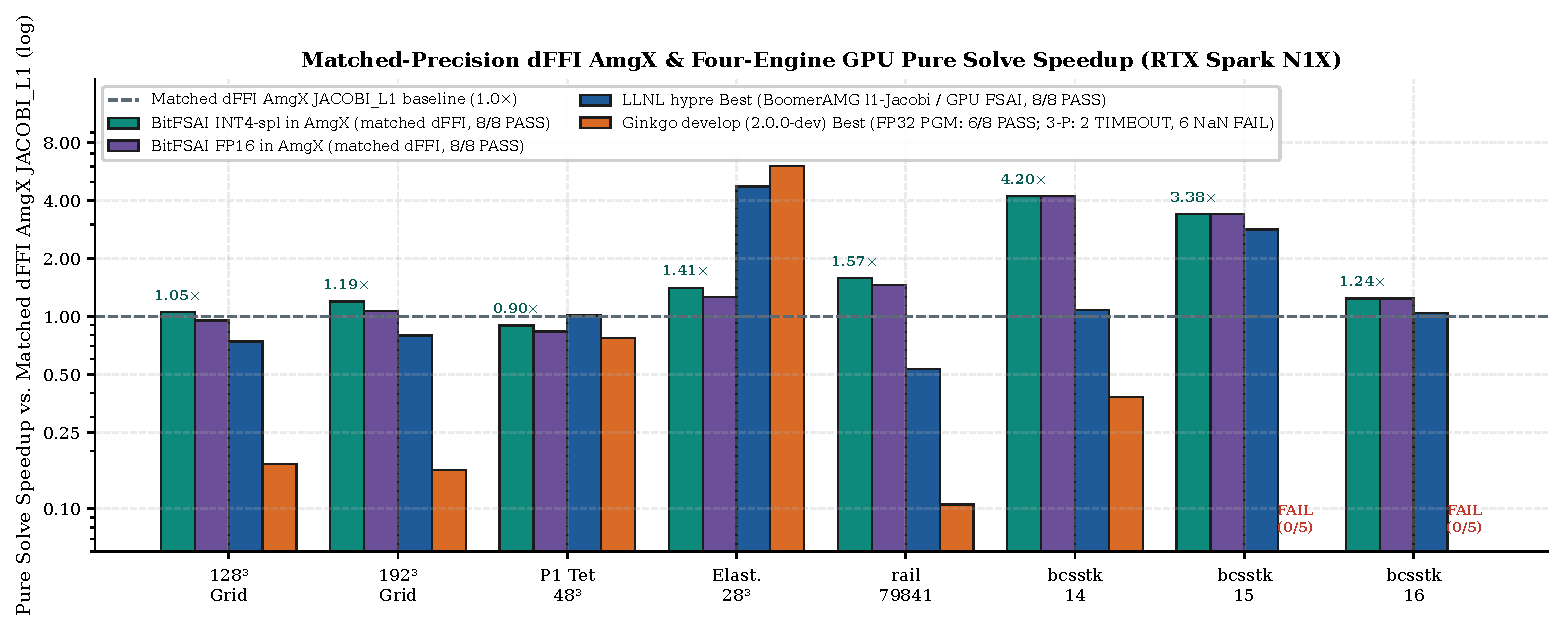
\includegraphics[width=\textwidth]{figures/fig2_four_engine_solve.pdf}
  \caption{Matched-precision \texttt{dFFI} AmgX and four-engine GPU pure-solve speedup relative to matched \texttt{dFFI} NVIDIA AmgX \texttt{JACOBI\_L1} (\texttt{mix\_jacobi}) on the RTX Spark N1X. BitFSAI \texttt{INT4-spl} (\texttt{dFFI}) passes 8/8 workloads at host \texttt{FP64} true residual $\le 7.86\times 10^{-9}$ ($1.19\times$--$4.20\times$ over matched \texttt{dFFI} \texttt{JACOBI\_L1} on 6/8 workloads; $1.05\times$ on $128^3$; $0.90\times$ on \texttt{tet48}). Our unscaled three-precision Ginkgo configuration (\texttt{mg\_isai\_3p}) produces \texttt{0/8} verified solutions (\texttt{TIMEOUT} at 240\,s on $128^3$/$192^3$, \texttt{0/5} \texttt{NaN} at 2000 iters on the other 6 workloads), and \texttt{FP32} \texttt{Pgm} fails \texttt{0/5} on \texttt{bcsstk15} and \texttt{bcsstk16}.}
  \label{fig:four_engine}
\end{figure}

\begin{table}[t]
\centering\scriptsize
\begin{tabular}{@{}lrcrrrr@{}}
\toprule
Workload & Ginkgo Best & Gko 3-P (unsc.) & \texttt{hypre} \texttt{FP64} (\texttt{l1}/\texttt{FSAI}) & AmgX \texttt{JAC\_L1} (\texttt{dFFI}/\texttt{dDDI}) & BitFSAI \texttt{INT4} (\texttt{dFFI}) & Spd (\texttt{dFFI} JAC / \texttt{hypre} / Gko) \\
\midrule
$128^3$ Grid (2.1M) & 842.4 (101) & TIMEOUT & 195.2 / 228.1 & 144.4 / 175.9 (18) & \textbf{137.5 (9)} & $1.05\times$ / $\mathbf{1.42\times}$ / $\mathbf{6.13\times}$ \\
$192^3$ Grid (7.1M) & 3585.3 (122) & TIMEOUT & 715.7 / 887.0 & 568.8 / 693.5 (19) & \textbf{477.1 (9)} & $\mathbf{1.19\times}$ / $\mathbf{1.50\times}$ / $\mathbf{7.51\times}$ \\
$P_1$ Tet $48^3$ & 68.5 (47) & FAIL (0/5) & \textbf{52.2} / 52.3 & 52.7 / 62.9 (54) & 58.9 (30) & $0.90\times$ / $0.89\times$ / $\mathbf{1.16\times}$ \\
Elasticity $28^3$ & \textbf{271.5}$^\dagger$ \textbf{(119)} & FAIL (0/5) & 644.6 / 345.4 & 1633.0 / 2034.0 (560) & 1161.0 (226) & $\mathbf{1.41\times}$ / $0.30\times$ / $0.23\times$ \\
\texttt{rail\_79841\_neg} & 61.8 (78) & FAIL (0/5) & 12.2 / 14.5 & 6.50 / 8.14 (18) & \textbf{4.13 (9)} & $\mathbf{1.57\times}$ / $\mathbf{2.95\times}$ / $\mathbf{15.0\times}$ \\
\texttt{bcsstk14} & 182.8 (307) & FAIL (0/5) & 114.0 / 64.4 & 69.7 / 72.7 (433) & \textbf{16.61 (63)} & $\mathbf{4.20\times}$ / $\mathbf{3.88\times}$ / $\mathbf{11.0\times}$ \\
\texttt{bcsstk15} & FAIL (0/5) & FAIL (0/5) & 256.5 / 65.1 & 183.5 / 208.1 (866) & \textbf{54.24 (138)} & $\mathbf{3.38\times}$ / $\mathbf{1.20\times}$ / n/a \\
\texttt{bcsstk16} & FAIL (0/5) & FAIL (0/5) & 22.3 / 14.9 & 15.5 / 18.0 (76) & \textbf{12.52 (36)} & $\mathbf{1.24\times}$ / $\mathbf{1.19\times}$ / n/a \\
\bottomrule
\end{tabular}
\caption{Median pure solve times in ms (outer \texttt{PCG} iterations in parentheses; for AmgX \texttt{JAC\_L1}, the count shown is \texttt{dFFI}, matching \texttt{dDDI} on 4/8 workloads while \texttt{dDDI} takes $558$ on \texttt{elastic28}, $432$ on \texttt{bcsstk14}, $867$ on \texttt{bcsstk15}, and $74$ on \texttt{bcsstk16}) across four GPU AMG engines on the RTX Spark N1X; fastest pure-solve engine per row is bolded (on $128^3$, \texttt{dFFI} \texttt{INT4-spl} and \texttt{dFFI} \texttt{JACOBI\_L1} are within our sub-$1.10\times$ overlapping-range parity rule, as are \texttt{hypre} \texttt{l1-Jacobi} and \texttt{dFFI} \texttt{JACOBI\_L1} on \texttt{tet48}). Every passing entry satisfies host \texttt{FP64} residual $\le 10^{-8}$ (\texttt{BitFSAI}: 0 recoveries in timed \texttt{step=2} trials, max residual $7.854\times 10^{-9}$). Cross-mode speedups of \texttt{dFFI} \texttt{INT4-spl} over stock \texttt{dDDI} \texttt{JACOBI\_L1} (combining cycle precision, custom outer \texttt{PCG} wrapper, and smoother changes) are $1.07\times$--$4.38\times$. $^\dagger$On \texttt{Elasticity 28$^3$}, Ginkgo \texttt{mg\_isai\_f32} pays $2416.7\text{ ms}$ cold setup ($2693.1\text{ ms}$ cold \texttt{setup + solve}, vs.\ $395.9\text{ ms}$ cold \texttt{setup + solve} for \texttt{hypre} \texttt{FSAI} and $2247.7\text{ ms}$ warm \texttt{resetup + solve} for BitFSAI in AmgX).}
\label{tab:four_engine}
\end{table}

\begin{table}[t]
\centering\scriptsize
\begin{tabular}{@{}lrrrrrr@{}}
\toprule
Workload & \texttt{dDDI} \texttt{JAC\_L1} (\texttt{slv}/\texttt{pair}) & \texttt{dDDI} \texttt{FP16} (\texttt{slv}/\texttt{pair}) & \texttt{dDDI} \texttt{INT4} (\texttt{slv}/\texttt{pair}) & \texttt{dFFI} \texttt{JAC\_L1} (\texttt{slv}/\texttt{pair}) & \texttt{dFFI} \texttt{FP16} (\texttt{slv}/\texttt{pair}) & \texttt{dFFI} \texttt{INT4} (\texttt{slv}/\texttt{pair}; $[\min\text{--}\max]$) \\
\midrule
$128^3$ Grid & 175.9 / 311.0 & 163.6 / 386.9 & 156.6 / 381.5 & 144.4 / \textbf{286.9} & 152.0 / 446.2 & \textbf{137.5} / 375.6 $[131.2\text{--}147.9]$ \\
$192^3$ Grid & 693.5 / 1178.5 & 603.0 / 1388.8 & 566.6 / 1376.0 & 568.8 / \textbf{1002.1} & 535.8 / 1387.9 & \textbf{477.1} / 1298.6 $[461.9\text{--}488.7]$ \\
$P_1$ Tet $48^3$ & 62.9 / 96.2 & 76.0 / 192.2 & 70.4 / 181.5 & \textbf{52.7 / 82.6} & 63.3 / 173.8 & 58.9 / 164.7 $[58.7\text{--}71.7]$ \\
Elasticity $28^3$ & 2034.0 / 2272.1 & 1533.1 / 2616.4 & 1451.7 / 2536.9 & 1633.0 / \textbf{1845.1} & 1302.5 / 2386.7 & \textbf{1161.0} / 2247.7 $[1141.6\text{--}1177.5]$ \\
\texttt{rail\_79841\_neg} & 8.14 / 18.34 & 6.31 / 22.47 & 6.10 / 23.17 & 6.50 / \textbf{16.50} & 4.46 / 19.07 & \textbf{4.13} / 19.18 $[4.08\text{--}4.39]$ \\
\texttt{bcsstk14} & 72.75 / 76.28 & 20.30 / 30.91 & 20.31 / 31.21 & 69.74 / 73.01 & \textbf{16.61 / 27.54} & \textbf{16.61} / 27.60 $[16.27\text{--}17.01]$ \\
\texttt{bcsstk15} & 208.06 / 214.31 & 55.50 / 72.91 & 57.97 / 74.65 & 183.53 / 188.73 & \textbf{54.03 / 70.31} & 54.24 / 70.32 $[54.15\text{--}54.95]$ \\
\texttt{bcsstk16} & 17.96 / 28.79 & 21.07 / 71.07 & 20.78 / 73.37 & 15.50 / \textbf{24.54} & \textbf{12.52} / 68.11 & \textbf{12.52} / 66.89 $[12.41\text{--}25.07]$ \\
\bottomrule
\end{tabular}
\caption{Matched-precision \texttt{dDDI} (\texttt{FP64} inner V-cycle) and matched-precision \texttt{dFFI} (\texttt{FP32} inner V-cycle, \texttt{FP64} outer \texttt{PCG}) median \texttt{solve / paired} times (ms) inside NVIDIA AmgX (100\% pass across all 8 workloads, zero recoveries in timed \texttt{step=2} trials, max residual $\le 7.87\times 10^{-9}$ across all smoothers and $\le 7.86\times 10^{-9}$ for \texttt{INT4-spl}; on untimed \texttt{warm} \texttt{step=0} $128^3$ and $192^3$ grids, all three \texttt{dFFI} smoothers triggered the $r^\top z$ guard and recovered cleanly via \texttt{dDDI}, logged in \texttt{summary.json}). Fastest \texttt{dFFI} solve and paired times per row are bolded.}
\label{tab:paired}
\end{table}

\begin{figure}[t]
  \centering
  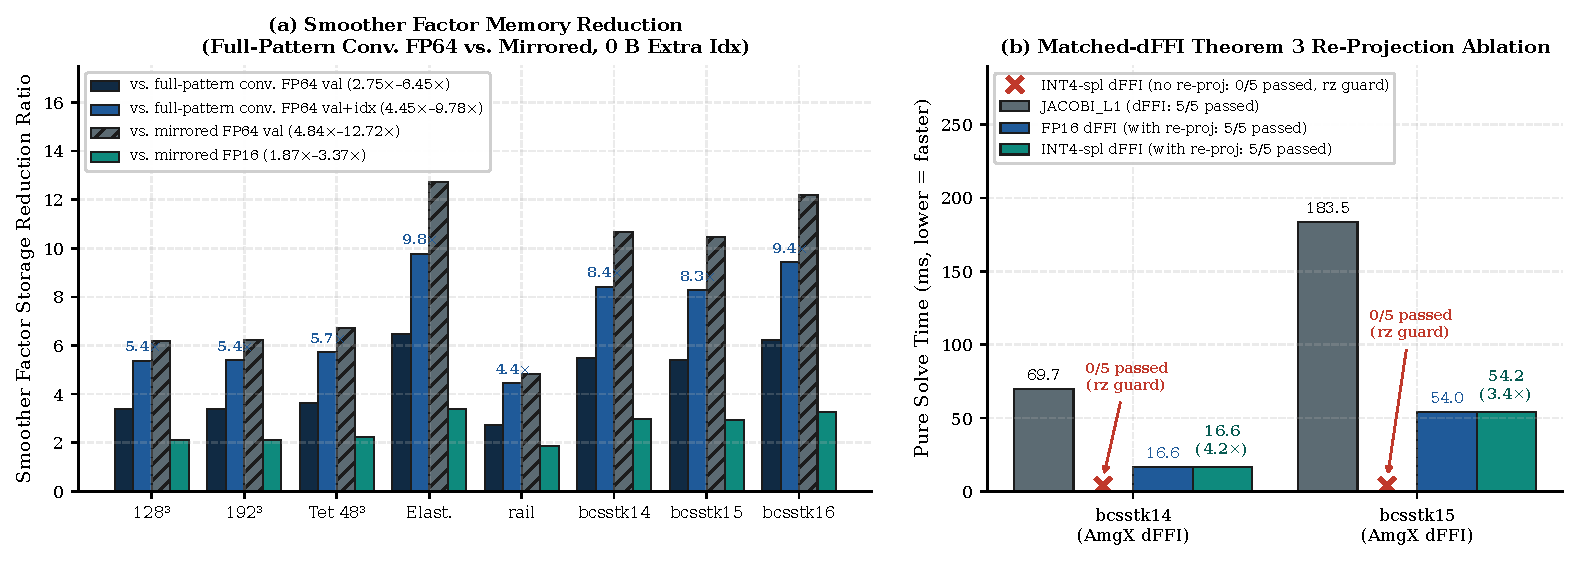
\includegraphics[width=\textwidth]{figures/fig3_memory_and_reproj.pdf}
  \caption{(a)~Persistent smoother factor storage reduction across all 8 workloads ($0\text{ B}$ extra CSR indices) relative to full-pattern lower-triangular \texttt{FP64} ($2.75\times$--$6.45\times$ values, $4.45\times$--$9.78\times$ values + \texttt{int32} indices) and mirrored \texttt{FP64}/\texttt{FP16} ($4.84\times$--$12.72\times$ / $1.87\times$--$3.37\times$); against a same-pattern $K \le 16$ conventional \texttt{FP64} factor (accounting for $K \le 16$ truncation on high-degree matrices), the reduction is $2.75\times$--$4.45\times$ (values) and $4.23\times$--$6.84\times$ (values + indices). (b)~Matched-precision \texttt{dFFI} AmgX Theorem~3 re-projection ablation on stiff structural matrices: disabling re-projection (\texttt{mix\_int4\_norep}) yields \texttt{0/5} passed on each matrix (all 5 triggered the $r^\top z$ guard and failed both stage~0 and stage~1), whereas enabling re-projection passes \texttt{5/5} with $4.20\times$ and $3.38\times$ speedup over matched \texttt{dFFI} \texttt{JACOBI\_L1}.}
  \label{fig:mem_reproj}
\end{figure}

Three findings stand out from the four-engine evaluation:
\begin{enumerate}
  \item \emph{Matched-precision (\texttt{dFFI} and \texttt{dDDI}) smoother performance and \texttt{dFFI} guard sensitivity inside the same hierarchy:} Holding the \texttt{PMIS-D2} hierarchy and inner-cycle precision fixed (Table~\ref{tab:paired}), in matched \texttt{dFFI} precision \texttt{BitFSAI INT4-spl} achieves clear pure-solve speedups of $\mathbf{1.19\times\text{--}4.20\times}$ over matched \texttt{dFFI} \texttt{JACOBI\_L1} on 6/8 workloads ($192^3$, \texttt{elastic28}, \texttt{rail\_79841\_neg}, \texttt{bcsstk14}, \texttt{bcsstk15}, \texttt{bcsstk16}), near-parity within overlapping ranges on $128^3$ ($137.5$ $[131.2\text{--}147.9]$ vs.\ $144.4\text{ ms}$ $[140.5\text{--}163.9]$, $1.05\times$), and $0.90\times$ on \texttt{tet48} ($58.9$ vs.\ $52.7\text{ ms}$); in paired \texttt{dFFI} \texttt{resetup + solve}, \texttt{INT4-spl} wins clearly on the two stiffest structural matrices ($2.65\times$ on \texttt{bcsstk14}, $2.68\times$ on \texttt{bcsstk15}), whereas diagonal \texttt{JACOBI\_L1} wins paired time on the other 6 workloads ($0.37\times$--$0.86\times$: $0.86\times$ on \texttt{rail\_79841\_neg}, $0.82\times$ on \texttt{elastic28}, $0.77\times$ on $192^3$, $0.76\times$ on $128^3$, $0.50\times$ on \texttt{tet48}, $0.37\times$ on \texttt{bcsstk16}), reflecting \texttt{BitFSAI}'s heavier per-resetup path (which includes CSR validation, per-row Cholesky factorization, and Kahan-compensated patch-energy verification; amortized over multiple right-hand sides on fixed operators). Against matched \texttt{dFFI} \texttt{BitFSAI FP16}, \texttt{INT4-spl} achieves clear pure-solve speedups on $128^3$ ($1.11\times$, $[131.2\text{--}147.9]$ vs.\ $[148.9\text{--}174.8]$), $192^3$ ($1.12\times$, $[461.9\text{--}488.7]$ vs.\ $[488.3\text{--}635.1]$), and \texttt{elastic28} ($1.12\times$, $[1141.6\text{--}1177.5]$ vs.\ $[1273.3\text{--}1306.0]$), and matches \texttt{FP16} within $0\%$--$8\%$ on the remaining 5 workloads ($1.00\times$--$1.08\times$ solve, $0.99\times$--$1.19\times$ paired across all 8) while storing $1.87\times$--$3.37\times$ less smoother memory. In matched \texttt{dDDI} precision, \texttt{INT4-spl} matches \texttt{FP16} within 0--4 iterations and $0.96\times$--$1.08\times$ solve time across all 8 workloads while beating \texttt{dDDI} \texttt{JACOBI\_L1} on 6/8 workloads ($1.12\times$--$3.59\times$). Combining the \texttt{dDDI}-to-\texttt{dFFI} cycle precision change with \texttt{INT4-spl} accelerates pure solve $1.07\times$--$4.38\times$ over stock \texttt{dDDI} \texttt{JACOBI\_L1} across all 8 workloads ($1.02\times$--$1.68\times$ vs.\ \texttt{dDDI} \texttt{FP16}); note that this cross-mode comparison also changes the outer \texttt{PCG} driver implementation (\texttt{dDDI} invokes AmgX's native \texttt{PCG} solver directly, whereas \texttt{dFFI} uses \texttt{bench\_amgx.cu}'s custom \texttt{FP64} outer \texttt{PCG} loop, \texttt{SpMV}, reductions, and stopping logic, which the matched-\texttt{dFFI} smoother comparisons above hold fixed). Crucially, while every timed (\texttt{step=2}) trial of the reprojected and Jacobi configurations across all 8 workloads ran with zero recoveries, on the separate untimed \texttt{warm} (\texttt{step=0}) $128^3$ (5/5) and $192^3$ (3/3) systems \emph{all three} \texttt{dFFI} smoothers (\texttt{mix\_jacobi}, \texttt{mix\_fp16\_rep}, \texttt{mix\_int4\_rep}) triggered the outer \texttt{PCG} $r^\top z$ curvature guard and fell back cleanly to \texttt{dDDI} (24 warm rows in \texttt{amgx\_8cases.csv}, e.g., $\approx 540\text{ ms}$ recovered \texttt{dFFI} vs.\ $\approx 157\text{ ms}$ plain \texttt{dDDI} on $128^3$ \texttt{step=0}), underscoring that mixed-precision \texttt{dFFI} inner V-cycles are inherently sensitive to \texttt{FP32} hierarchy asymmetry and require the outer $r^\top z$ guard and \texttt{dDDI} fallback regardless of smoother.
  \item \emph{Necessity of Theorem~3 re-projection for the guarded \texttt{dFFI} pipeline:} Figure~\ref{fig:mem_reproj}b isolates Theorem~3 inside matched-precision \texttt{dFFI} AmgX on \texttt{bcsstk14} and \texttt{bcsstk15}. Disabling re-projection in \texttt{dFFI} (\texttt{mix\_int4\_norep}) results in \texttt{0/5} passed on each matrix because the driver aborts on $r^\top z \le 0$: stage~0 (\texttt{dFFI}) triggers the $r^\top z$ guard at iteration~1, \texttt{bench\_amgx.cu} sets \texttt{recovered=1} to attempt stage-1 \texttt{dDDI} recovery with the same unprojected smoother, and stage~1 also aborts on $r^\top z$ (total 1--2 iterations, final residuals $6.53$ and $25.2$, \texttt{pass=0}). Under AmgX's built-in \texttt{dDDI} \texttt{PCG} (\texttt{int4\_norep}), the same unprojected smoother still passes \texttt{5/5}, increasing \texttt{bcsstk14} from $63$ iterations ($20.31\text{ ms}$) to $69$ iterations ($22.32\text{ ms}$) and degrading \texttt{bcsstk15} from $138$ iterations ($57.97\text{ ms}$) to $309$ iterations ($125.89\text{ ms}$, $2.17\times$ slower). Enabling Theorem~3 re-projection restores \texttt{5/5} \texttt{dFFI} convergence ($16.61\text{ ms}$ and $54.24\text{ ms}$) with zero recoveries.
  \item \emph{Complete solver configurations across libraries:} Comparing full solver configurations across engines, AmgX with \texttt{dFFI} BitFSAI (\texttt{FP32} inner cycle, $8\times 10^{-9}$ inner stop) is the fastest engine in pure solve on 6 of 8 workloads ($128^3$, $192^3$, \texttt{rail\_79841\_neg}, \texttt{bcsstk14}, \texttt{bcsstk15}, \texttt{bcsstk16}), beating \texttt{hypre} \texttt{BoomerAMG}'s full-\texttt{FP64} best configuration ($7\times 10^{-9}$ inner stop) by $1.19\times$--$3.88\times$ (including $1.42\times$ on $128^3$ with non-overlapping ranges $[131.2\text{--}147.9]$ vs.\ $[184.6\text{--}207.9]$, while within AmgX \texttt{dFFI} on $128^3$, \texttt{INT4-spl} $137.5\text{ ms}$ and \texttt{JACOBI\_L1} $144.4\text{ ms}$ are at parity; similarly within AmgX \texttt{dFFI} on \texttt{bcsstk14}/\texttt{bcsstk15}/\texttt{bcsstk16}, \texttt{INT4-spl} and \texttt{BitFSAI FP16} are at parity, with \texttt{FP16} posting median $54.03\text{ ms}$ vs.\ \texttt{INT4-spl} $54.24\text{ ms}$ on \texttt{bcsstk15} under overlapping ranges). Because \texttt{hypre} runs its inner V-cycle entirely in \texttt{FP64}, those \texttt{dFFI} ratios combine precision, hierarchy, outer-loop, and smoother differences; at matched \texttt{FP64} inner precision (\texttt{dDDI} BitFSAI vs.\ \texttt{FP64} \texttt{hypre} best, Table~\ref{tab:paired}), \texttt{dDDI} BitFSAI still beats \texttt{hypre} on $128^3$ ($156.6$ vs.\ $195.2\text{ ms}$), $192^3$ ($566.6$ vs.\ $715.7\text{ ms}$), \texttt{rail\_79841\_neg} ($6.10$ vs.\ $12.2\text{ ms}$), \texttt{bcsstk14} ($20.31$ vs.\ $64.4\text{ ms}$), and \texttt{bcsstk15} ($57.97$ vs.\ $65.1\text{ ms}$, $1.12\times$), while trailing \texttt{hypre} on \texttt{tet48} ($70.4$ vs.\ $52.2\text{ ms}$), \texttt{elastic28} ($1451.7$ vs.\ $345.4\text{ ms}$), and \texttt{bcsstk16} ($20.78$ vs.\ $14.9\text{ ms}$). On $P_1$ \texttt{Tet 48$^3$}, \texttt{hypre} \texttt{BoomerAMG} (\texttt{PMIS} + \texttt{ext+i} + \texttt{l1-Jacobi}, $52.2\text{ ms}$, $[50.2\text{--}52.8]$) and AmgX \texttt{dFFI} \texttt{JACOBI\_L1} ($52.7\text{ ms}$, $[51.6\text{--}57.0]$) are at parity under our sub-$1.10\times$ overlapping-range rule, both ahead of \texttt{dFFI} BitFSAI ($58.9\text{ ms}$). On \texttt{Elasticity 28$^3$}, Ginkgo's \texttt{mg\_isai\_f32} (\texttt{Pgm} + \texttt{SpdIsai} + \texttt{FP32} cycle) achieves the fastest pure solve ($271.5\text{ ms}$, $119$ iters, ahead of \texttt{hypre} \texttt{FSAI} at $345.4\text{ ms}$, $174$ iters, and scalar \texttt{PMIS-D2} AmgX with BitFSAI at $1161.0\text{ ms}$, $226$ iters), though Ginkgo pays $2416.7\text{ ms}$ of cold hierarchy/ISAI setup ($2693.1\text{ ms}$ cold \texttt{setup + solve}, vs.\ $395.9\text{ ms}$ cold \texttt{setup + solve} for \texttt{hypre} \texttt{FSAI} and $2247.7\text{ ms}$ warm \texttt{resetup + solve} for BitFSAI in AmgX). For Ginkgo, our unscaled three-precision configuration (\texttt{mg\_isai\_3p}, storing coarse levels in unscaled \texttt{FP16} rather than the scaled setup of~\cite{tsai2023three}, which overflows on \texttt{bcsstk} entries reaching $10^{10}$) produces \texttt{0/8} verified solutions (2 timeouts at the 240\,s cap on $128^3$ and $192^3$, recorded as \texttt{trial=-1, note=timeout}, and \texttt{0/5} \texttt{NaN} residuals at 2000 iterations on the remaining 6 workloads); \texttt{mg\_jacobi\_f32} fails \texttt{0/5} on \texttt{elastic28}, \texttt{bcsstk14}, \texttt{bcsstk15}, and \texttt{bcsstk16} (and passes \texttt{4/5} on \texttt{tet48}); and \texttt{mg\_isai\_f32} fails \texttt{0/5} (\texttt{NaN} at 2000 iterations) on \texttt{bcsstk15} and \texttt{bcsstk16}.
\end{enumerate}

\subsection{GPU Silicon Evaluation of \texttt{FP8 E5M2} Coarse Operators and Sparse-Depth Polynomial Boosting}\label{sec:multilevel_eval}
Table~\ref{tab:multilevel_gpu} and Figure~\ref{fig:gpu_multilevel} evaluate \texttt{standalone\_amg.cu} in \texttt{int4}-only allocation mode (\texttt{benchmarks/results/standalone\_multilevel.csv}) on $128^3$ (2.10M unknowns) and $192^3$ (7.08M unknowns), combining SDDM- and normal-range-guarded \texttt{FP8 E5M2} row-sum-repaired coarse operators with sparse-depth polynomial boosting inside CUDA Graphs.

\begin{table}[t]
\centering\scriptsize
\begin{tabular}{@{}llrrrrrr@{}}
\toprule
Grid & Multilevel Configuration & Iters & Resetup & Solve $[\min\text{--}\max]$ & Paired $[\min\text{--}\max]$ & Solve / Paired Spd & Stored Buf. \\
\midrule
$128^3$ & V-cycle + \texttt{FP32} coarse $A_c$ (base) & 24 & 106.4 & 404.3 $[393.9\text{--}412.2]$ & 510.7 $[497.1\text{--}520.7]$ & $1.00\times$ / $1.00\times$ & 173.6 MiB \\
$128^3$ & V-cycle + \textbf{\texttt{FP8 E5M2}} guarded $A_c$ & 25 & 235.0 & 386.7 $[368.7\text{--}472.8]$ & 624.8 $[597.5\text{--}819.2]$ & $1.05\times$ / $0.82\times$ & \textbf{119.2 MiB} \\
$128^3$ & \texttt{Poly4} ($j\%4=0$, $t=1.25$) + \texttt{FP32} & \textbf{10} & \textbf{95.7} & 380.8 $[379.7\text{--}382.5]$ & 477.1 $[475.5\text{--}479.1]$ & $1.06\times$ / $1.07\times$ & 173.6 MiB \\
$128^3$ & \textbf{\texttt{Poly4@2}} ($j\%4=2$, $t=1.25$) + \texttt{FP32} & 12 & 99.8 & \textbf{297.6} $[294.6\text{--}368.4]$ & \textbf{394.4} $[392.2\text{--}478.9]$ & $\mathbf{1.36\times}$ / $\mathbf{1.29\times}$ & 173.6 MiB \\
$128^3$ & \textbf{\texttt{Poly4@2} + \texttt{FP8 E5M2} guarded $A_c$} & 13 & 224.9 & 330.4 $[321.4\text{--}345.8]$ & 570.7 $[544.8\text{--}575.2]$ & $\mathbf{1.22\times}$ / $0.89\times$ & \textbf{119.2 MiB} \\
\midrule
$192^3$ & V-cycle + \texttt{FP32} coarse $A_c$ (base) & 28 & 327.7 & 1511.1 $[1483.1\text{--}1521.5]$ & 1833.3 $[1810.8\text{--}3087.4]$ & $1.00\times$ / $1.00\times$ & 589.8 MiB \\
$192^3$ & V-cycle + \textbf{\texttt{FP8 E5M2}} guarded $A_c$ & 28 & 1177.5 & 1404.4 $[1390.5\text{--}1407.0]$ & 2568.1 $[2445.0\text{--}2900.4]$ & $1.08\times$ / $0.71\times$ & \textbf{405.0 MiB} \\
$192^3$ & \texttt{Poly4} ($j\%4=0$, $t=1.25$) + \texttt{FP32} & \textbf{10} & 326.4 & 1165.0 $[1137.8\text{--}1190.2]$ & 1491.4 $[1460.5\text{--}1520.1]$ & $\mathbf{1.30\times}$ / $\mathbf{1.23\times}$ & 589.8 MiB \\
$192^3$ & \texttt{Poly4@2} ($j\%4=2$, $t=1.25$) + \texttt{FP32} & 13 & \textbf{321.3} & 1022.3 $[1022.2\text{--}1026.7]$ & \textbf{1347.9} $[1338.3\text{--}1348.1]$ & $\mathbf{1.48\times}$ / $\mathbf{1.36\times}$ & 589.8 MiB \\
$192^3$ & \textbf{\texttt{Poly4@2} + \texttt{FP8 E5M2} guarded $A_c$} & 13 & 784.3 & \textbf{990.4} $[982.8\text{--}993.8]$ & 1773.1 $[1767.1\text{--}1834.9]$ & $\mathbf{1.53\times}$ / $1.03\times$ & \textbf{405.0 MiB} \\
\bottomrule
\end{tabular}
\caption{GPU silicon evaluation of SDDM- and normal-range-guarded row-sum-repaired \texttt{FP8 E5M2} coarse operators and sparse-depth polynomial boosting in \texttt{reference/standalone\_amg.cu} (\texttt{int4}-only mode, times in ms with $[\min\text{--}\max]$ trial ranges, 100\% pass at timed host \texttt{FP64} true residual $\le 6.49\times 10^{-9}$). \emph{Stored Buf.} (\texttt{resident\_bytes} = \texttt{weight\_bytes + coarse\_bytes} in \texttt{int4}-only mode) measures resident smoother-factor and nonterminal coarse apply-value buffers, distinct from total process GPU VRAM (which also retains \texttt{FP64} $A_\ell$ on all levels, CSR indices, workspaces, transfer/\texttt{RAP}, and outer \texttt{PCG} vectors).}
\label{tab:multilevel_gpu}
\end{table}

\begin{figure}[t]
  \centering
  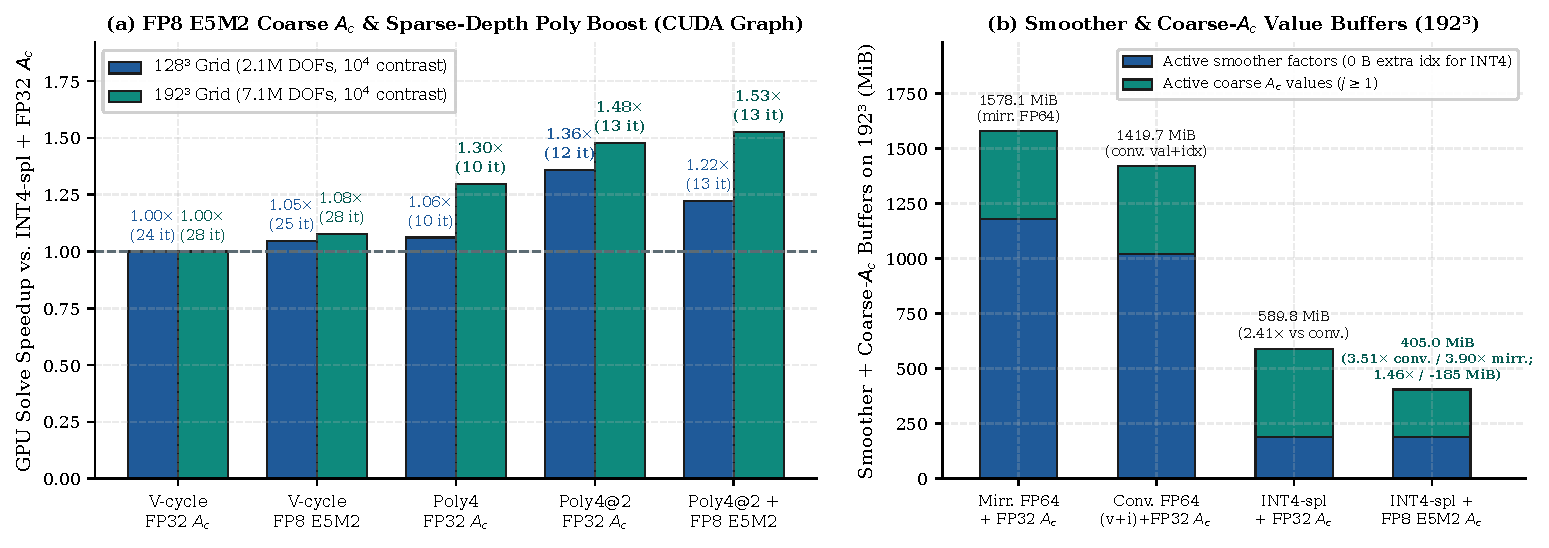
\includegraphics[width=\textwidth]{figures/fig4_gpu_multilevel.pdf}
  \caption{Multilevel SDDM- and normal-range-guarded \texttt{FP8 E5M2} coarse operators and sparse-depth polynomial boosting on $10^4$-contrast 3D grids. (a)~GPU solve speedup vs.\ \texttt{INT4-spl} + \texttt{FP32} $A_c$ V-cycle, reaching $1.53\times$ faster solve on $192^3$ ($28 \to 13$ iterations) and $1.36\times$ (\texttt{poly4@2}) / $1.22\times$ (\texttt{poly4@2 + FP8}) on $128^3$. (b)~$192^3$ stored smoother-factor and coarse-$A_c$ apply-value buffers: \texttt{INT4-spl} + guarded \texttt{FP8 E5M2} ($405.0\text{ MiB}$) achieves a $3.51\times$ reduction vs.\ conventional lower-triangular \texttt{FP64} (values + indices) + \texttt{FP32} $A_c$ ($1419.7\text{ MiB}$), $3.90\times$ vs.\ mirrored \texttt{FP64} + \texttt{FP32} $A_c$ ($1578.1\text{ MiB}$), and $1.46\times$ ($184.82\text{ MiB}$ saved) vs.\ \texttt{INT4-spl} + \texttt{FP32} $A_c$ ($589.8\text{ MiB}$).}
  \label{fig:gpu_multilevel}
\end{figure}

Both mechanisms yield clear storage and solve-time benefits on Blackwell silicon while enforcing the full normal-range \texttt{FP8 E5M2} and grounded-SDDM contract. On these 2-column Galerkin hierarchies, coarse levels satisfying nonpositive off-diagonals, the normal \texttt{E5M2} range $[2^{-14}, 57344]$, and component grounding run in \texttt{FP8 E5M2}, while levels violating those checks automatically fall back to \texttt{FP32} \texttt{af} and free their \texttt{FP8} buffers (\texttt{standalone\_multilevel.csv} records the resulting aggregate \texttt{coarse\_bytes}---$1.86\times$ smaller than all-\texttt{FP32}, reflecting partial per-level \texttt{FP32} fallback rather than an all-level $\approx 3.1\times$ bound---without a per-level \texttt{FP8} count column). On both $128^3$ and $192^3$, guarded \texttt{FP8 E5M2} cuts coarse $A_c$ apply-value buffers by $\mathbf{1.86\times}$ ($117.6\text{ MiB} \to 63.3\text{ MiB}$, saving $54.36\text{ MiB}$ on $128^3$; $400.6\text{ MiB} \to 215.8\text{ MiB}$, saving $184.82\text{ MiB}$ on $192^3$), reducing resident smoother-factor plus nonterminal coarse apply-value buffers by $\mathbf{1.46\times}$ on both grids ($173.6 \to 119.2\text{ MiB}$ on $128^3$; $589.8 \to 405.0\text{ MiB}$ on $192^3$) with zero extra iterations on $192^3$ ($28$ vs.\ $28$, $1.08\times$ solve) and 1 extra iteration on $128^3$ ($25$ vs.\ $24$, $1.05\times$ solve). Between the \texttt{FP8} and \texttt{FP32} configurations, the observed resetup difference is $\approx 125\text{ ms}$ on $128^3$ and $\approx 460\text{--}850\text{ ms}$ on $192^3$ (reflecting \texttt{build\_fp8\_coarse}'s device-to-host transfer, decoding, and host-side connected-component grounding verification on every numeric resetup---amortizing over multi-RHS solves on fixed operators while making \texttt{poly4@2 + FP32} fastest in single-solve paired time). Adding sparse-depth polynomial boosting at stride 4 (\texttt{poly4:1.25}) cuts outer iterations $2.80\times$ ($28 \to 10$) for a $1.30\times$ solve speedup ($1.23\times$ paired) on $192^3$; shifting the boost two levels deeper (\texttt{poly4@2:1.25}) avoids doubling level-1 work while cutting iterations $2.15\times$ ($28 \to 13$), raising \texttt{FP32}-$A_c$ speedup to $1.48\times$ solve and $1.36\times$ paired ($1347.9\text{ ms}$, $[1338.3\text{--}1348.1]$; $1.36\times$ solve and $1.29\times$ paired on $128^3$). Combining \texttt{poly4@2:1.25} with guarded \texttt{FP8 E5M2} coarse operators delivers the fastest pure solve on $192^3$ at $\mathbf{990.4\text{ ms}}$ ($\mathbf{1.53\times}$, 3-trial range $[982.8\text{--}993.8]$; paired $1773.1\text{ ms}$, $1.03\times$, which is parity under our sub-$1.10\times$ overlapping-range rule) versus the \texttt{INT4-spl} + \texttt{FP32} $A_c$ baseline across separate invocations of the same binary in \texttt{int4}-only mode (while \texttt{standalone\_8cases.csv} uses multi-method mode---where the $192^3$ \texttt{INT4} V-cycle ran in $1537.7\text{ ms}$ vs.\ $1511.1\text{ ms}$ here at identical $28$ iterations---so we restrict speedup claims to matched within-suite baselines), while combined active smoother + coarse-$A_c$ storage shrinks $3.51\times$ relative to conventional lower-triangular \texttt{FP64} (values + indices) + \texttt{FP32} $A_c$ ($1419.7\text{ MiB} \to 405.0\text{ MiB}$, or $3.90\times$ vs.\ mirrored \texttt{FP64} + \texttt{FP32} $A_c$, Figure~\ref{fig:gpu_multilevel}b).

\section{Asymptotic Multilevel Guarantees and Fundamental Limits}\label{sec:theory}
We now establish the formal multilevel convergence guarantees and fundamental precision limits of quantized AMG hierarchies---including variable coefficients, arbitrary weight contrast, nonzero \texttt{FP8 E5M2} coarse rounding at every level, and sub-4-bit / frozen-word bounds. All 44 multilevel, bit-limit, and drift theorems in this section are machine-checked in Lean~4 + Mathlib (\texttt{proofs/lean/Bitfsai/Multilevel.lean} [28] and \texttt{Bitfsai/BitLimits.lean} [16]) and cross-checked by 120 Z3 exact-real UNSAT obligations plus 9 SAT negative controls (\texttt{proofs/z3/verify\_multilevel\_z3.py} and \texttt{proofs/z3/verify\_bit\_limits\_z3.py}); the remaining graph-to-recurrence and finite-grid primitive steps of Theorems~7--8 and written network/entropy derivations of Theorem~9 are verified with explicit mechanization boundaries audited in Section~\ref{sec:audit}.

\subsection{Certified Damping Guard, Galerkin Sandwich, and Overdamping Obstruction}
Row-wise unit $A$-energy (Theorem~3) controls $(G_q A G_q^\top)_{ii} = 1$, but does not alone bound $\lambda_{\max}(G_q A G_q^\top) < 2/\omega$ for general sparsity patterns (the $3\times 3$ SPD Gram matrix with unit diagonal and off-diagonals $0.99$ has $\lambda_{\max} = 2.98 > 25/9$). An explicit three-pass entrywise bound certifies both SPDness and, under a Galerkin coarse sandwich, the upper Loewner bound $B_\ell \preceq A_\ell^{-1}$.

\begin{theorem}[Three-Pass Certified Damping Guard and Galerkin V-Cycle Sandwich]
For any finite SPD matrix $A_\ell$, full-column-rank prolongation $P_\ell$, and lower-triangular factor $G_\ell$ with positive diagonals ($M_\ell = G_\ell^\top G_\ell$), define
\[
  U_\ell = \max_i \bigl(|G_\ell|\,|A_\ell|\,|G_\ell|^\top \mathbf{1}\bigr)_i, \qquad
  \omega_\ell = \min\!\left(\frac{18}{25}, \frac{1}{U_\ell}\right), \qquad
  R_\ell = \omega_\ell M_\ell,
\]
computed in three sparse matrix-vector products. Because $\lambda_{\max}(G_\ell A_\ell G_\ell^\top) \le \|G_\ell A_\ell G_\ell^\top\|_\infty \le U_\ell$, we have $0 \prec R_\ell \preceq A_\ell^{-1}$ (with scalar smoothing gain $h \le 1 - (1-h)^2$ for $h \in [0,1]$, \texttt{guarded\_smoothing\_scalar}). Consequently, if the coarse operator $\tilde{A}_{\ell+1}$ satisfies the explicit Galerkin lower sandwich $\gamma_\ell (P_\ell^\top A_\ell P_\ell) \preceq \tilde{A}_{\ell+1}$ ($\gamma_\ell > 0$, including exact unrounded $\tilde{A}_{\ell+1} = P_\ell^\top A_\ell P_\ell$ at $\gamma_\ell = 1$) and $B_{\ell+1} = B_{\ell+1}^\top$ satisfies $0 \preceq B_{\ell+1} \preceq \tilde{A}_{\ell+1}^{-1}$, then $T_\ell = P_\ell^\top A_\ell P_\ell$ and $\tilde{A}_{\ell+1}$ are SPD, $\gamma_\ell \tilde{A}_{\ell+1}^{-1} \preceq T_\ell^{-1}$, and the symmetric two-level V-cycle operator
\[
  B_\ell = 2 R_\ell - R_\ell A_\ell R_\ell + \gamma_\ell (I - R_\ell A_\ell) P_\ell B_{\ell+1} P_\ell^\top (I - A_\ell R_\ell)
\]
satisfies $B_\ell^\top = B_\ell$ and $0 \prec R_\ell \preceq B_\ell \preceq A_\ell^{-1}$ in arbitrary finite dimensions (\texttt{vcycle\_upper\_bound\_of\_galerkin\_sandwich}). In particular, for SDDM Galerkin operators $A_c = P^\top A P$ rounded symmetrically with relative edge error at most $u$ ($u = 1/8$ for normal-range \texttt{FP8 E5M2}) and exact row-sum repair, summing the per-edge scalar inequality $(1-u)w_{ij} \le \tilde{w}_{ij} \le (1+u)w_{ij}$ (Z3 \texttt{e5m2\_coarse\_sandwich}, which checks the scalar edge bound given the relative rounding premise) over graph edges yields $(1-u)A_c \preceq \tilde{A}_c \preceq (1+u)A_c$, so applying \texttt{vcycle\_upper\_bound\_of\_galerkin\_sandwich} with $\gamma = 1 - u = 7/8$ preserves $B_\ell \preceq A_\ell^{-1}$ at every finite depth; the accompanying W-cycle fixed-point ratio $\alpha = ((1-u)/(1+u))^2 = 49/81 > 1/2$ and defect-cycle matrix contraction are mechanized in \texttt{fp8\_e5m2\_wcycle\_constants} and \texttt{defect\_cycle\_matrix\_reduction}. (As noted in Section~\ref{sec:gpu_alg}, \texttt{standalone\_amg.cu}'s GPU \texttt{fp8coarse} path uses heuristic damping and unscaled $\gamma = 1$ coarse corrections rather than this certified $\gamma = 7/8$ scheme.)
\end{theorem}

We implement Theorem~5 in \texttt{reference/certified\_damping.hpp} using upward-rounded IEEE binary64 arithmetic (\texttt{std::nextafter}, checking \texttt{FE\_TONEAREST}, gradual underflow, symmetry $A = A^\top$, and positive diagonals; caller supplies SPDness of $A$), together with a \texttt{make\_int4\_split\_factor} / \texttt{make\_int4\_split\_factor\_from\_packed\_csr} adapter that certifies real downloaded \texttt{BitFSAI INT4\_Split} factors (verified directly against GPU apply in \texttt{reference/test\_bitfsai.cu}) and a downward-rounded \texttt{certified\_damping\_f32} helper (\texttt{bitfsai.cuh::apply} accepts \texttt{double damp} directly). However, an entrywise absolute-value guard alone can overdamp high-contrast chains: on $A = \bigl[\begin{smallmatrix}1 & -1\\ -1 & 1+s\end{smallmatrix}\bigr]$ ($s > 0$), the exact inverse factor $G = \bigl[\begin{smallmatrix}1 & 0\\ s^{-1/2} & s^{-1/2}\end{smallmatrix}\bigr]$ satisfies $G A G^\top = I$, yet in 1-based indexing $(|G|\,|A|\,|G|^\top)_{22} = (4+s)/s$ (0-based index \texttt{(1, 1)} in Lean's \texttt{Fin 2}), forcing $\omega \le s/(4+s) \to 0$ as $s \to 0^+$ (\texttt{absolute\_guard\_overdamping\_witness}). Contrast-independent convergence therefore requires tracking upper damping and fine-space smoothing jointly.

\subsection{Monotone Effectiveness Recurrence and the Work-Convergence Frontier}
\begin{theorem}[Monotone One-Level Effectiveness Recurrence and Product-Inequality Frontier]
Let $A$ be SPD, $P$ have full column rank, $T = P^\top A P$, $0 \preceq R \preceq A^{-1}$ be symmetric, $S = I - R A$, and let symmetric coarse operator $B_{\mathrm{amp}}$ satisfy the damped sandwich $\alpha g(e) T^{-1} \preceq \gamma B_{\mathrm{amp}} \preceq T^{-1}$ ($\gamma > 0$, $\alpha, g(e) \ge 0$; arising from $l T \preceq A_c \preceq h T$ with $\gamma = l$, $\alpha = l/h$, and a child polynomial correction with energy gain in $[g(e), 1]$). Suppose the weak approximation and smoothing inequality holds in $A^{-1}$ dual form:
\[
  S (A^{-1} - P T^{-1} P^\top) S^\top \preceq \zeta S A^{-1} S^\top + K (A^{-1} - S A^{-1} S^\top), \qquad 0 \le \zeta < 1, \quad K \ge 0
\]
(equivalently $S_{\mathrm{sym}} Q S_{\mathrm{sym}} \preceq \zeta S_{\mathrm{sym}}^2 + K (I - S_{\mathrm{sym}}^2)$ in $A^{1/2}$-symmetrized coordinates). Then the two-level preconditioner $B_{\mathrm{level}} = 2 R - R A R + \gamma S P B_{\mathrm{amp}} P^\top S^\top$ is symmetric, satisfies the exact coarse comparison step $A^{-1} - B_{\mathrm{level}} \preceq (1 - c) S A^{-1} S^\top + c S (A^{-1} - P T^{-1} P^\top) S^\top$ with $c = \min(\alpha g(e), 1/(K + 1 - \zeta))$, and obeys the two-sided Loewner effectiveness sandwich $e_{\mathrm{new}} A^{-1} \preceq B_{\mathrm{level}} \preceq A^{-1}$ with
\[
  e_{\mathrm{new}} = \min\!\left(p\,g(e),\, d\right), \qquad p = \alpha(1-\zeta), \qquad d = \frac{1-\zeta}{K + 1 - \zeta}
\]
mechanized directly in arbitrary finite dimension without matrix square roots (\texttt{monotone\_effectiveness\_operator}, alongside \texttt{monotone\_effectiveness\_scalar} and \texttt{monotone\_effectiveness\_matrix}). Via weighted Young's inequality ($\tau > 0$), the approximation bound follows from a fine-space smoother lower bound $\eta Q_\star \preceq H$ and an approximate-lifting defect $\|Q v\|_2 \le \|Q_\star v\|_2 + \sqrt{\epsilon}\|(I - Q_\star)v\|_2$, giving $\zeta = (1 + 1/\tau)\epsilon$ and $K = (1+\tau)/(2\eta)$. For degree-$m$ Chebyshev acceleration~\cite{axelsson1989amli,notay2008kcycle,napov2012amli}, $\phi_m(e) = \tanh^2(m \operatorname{artanh}(\sqrt{e})) \sim m^2 e$ as $e \to 0$, and for degree-two Richardson at fixed scale $t$, concavity of $1 - (1 - t x)^2$ bounds the gain on $[u,1]$ by its smaller endpoint (\texttt{two\_call\_concave\_endpoint\_min}). Finally, for geometric level contraction $0 < \beta < 1$ and retention $0 < p < 1$, a positive periodic degree schedule $m_0,\dots,m_{k-1}$ simultaneously satisfies the linear-work product inequality $\prod_{i=0}^{k-1}(\beta m_i) < 1$ and super-unit gain product inequality $\prod_{i=0}^{k-1}(p m_i^2) > 1$ if and only if $\beta^2 < p$: no real positive schedule exists when $p \le \beta^2$ (\texttt{work\_convergence\_frontier}, \texttt{work\_convergence\_frontier\_periodic}), whereas whenever $\beta^2 < p$ there exist integers $k \ge 1, m \ge 2$ such that $(1,\dots,1,m)$ achieves $\beta^k m < 1$ and $p^k m^2 > 1$ (\texttt{work\_convergence\_frontier\_converse}).
\end{theorem}

This $\beta^2 < p$ characterization governs feasibility of the asymptotic work/gain product inequalities; turning a feasible schedule into uniform multilevel convergence additionally requires the per-level spectral sandwich ($l T \preceq A_c \preceq h T$) and smoothing/lifting bound of Theorem~6, which we construct for certified grounded SDDM hierarchies in Theorem~7. Our GPU \texttt{poly4} / \texttt{poly4@2} experiments (Section~\ref{sec:multilevel_eval}) are empirically motivated by this sparse-depth boost mechanism rather than a certified $\beta^2 < p$ bound on the heuristic \texttt{PMIS}/aggregation coarsener.

\subsection{Uniform Four-Phase Quantized Convergence for Grounded SDDM Matrices}
\begin{theorem}[Uniform Four-Phase Quantized Convergence for Grounded SDDM Matrices]
Let $A_0$ be any SPD grounded SDDM matrix with $n$ vertices and $m$ nonzero off-diagonal edges. At each nonterminal level:
\begin{enumerate}
  \item \emph{Linear-time fine-set selection:} conditional expectations of the quadratic potential $\Phi(x) = \sum_i x_i(1 - \sum_{j \neq i}(-A_{ij})x_j/(\delta d_i))$ select $F$ with internal incident weight at most $\delta d_i$ ($\delta = 3/4$) and $|F| \ge \lceil 3n/16\rceil$, giving size contraction $\beta \le 13/16$. Maintaining each undecided vertex's marginal potential change $\Delta_v = 1 - \sum_{u \neq v}(-A_{vu})x_u/(\delta d_v) - \sum_{u \neq v} x_u(-A_{uv})/(\delta d_u)$ and updating only incident neighbors when $x_v \leftarrow \in \{0,1\}$ runs in $O(\deg(v))$ per decision, totaling $O(m+n)$ operations (implemented in \texttt{select\_fine\_set\_incremental} and verified bit-for-bit identical to the dense $O(n^3)$ oracle across all levels in \texttt{verify\_sddm\_cycle.py}).
  \item \emph{Matrix-free Jacobi lifting:} initialize $F$ with the normalized external coarse/ground weighted mean and run 16 fixed Jacobi sweeps on $L_F = D - Z$, giving lifting defect $\epsilon = 7(3/4)^{32} < 1/1024$ and $T_\star \preceq P^\top A P \preceq (1+\epsilon)T_\star$.
  \item \emph{Sparsified range-extended 3-significand-bit (\texttt{FP8 E5M2}-width) coarse operator:} construct a linear-size spectral sparsifier~\cite{durfee2017schur,lee2015sparsification} within $1 \pm 1/128$ of the Schur complement $T_\star$ in near-linear randomized setup time (optionally via a 48-term truncated path expansion carrying an extra $63/64$ factor), round each positive edge and ground weight to a range-extended 3-significand-bit floating-point format (E5M2 significand width with relative error at most $u = 1/8$ across arbitrary dyadic exponents, as distinguished from 1-byte hardware \texttt{FP8 E5M2}'s $[2^{-14}, 57344]$ normal range), and derive diagonals from incident weights. This yields $l = (7/8)(127/128)/(1 + 1/1024)$ and $h = (9/8)(129/128)$ (scaling $l$ by $63/64$ if path-truncated), with coarse correction scale $\gamma = l$.
  \item \emph{Certified smoother (two realizations):} either (a)~the \emph{protected smoother} $R = (R_B + J_F D^{-1} J_F^\top/(1+\delta))/2$ using any upper-certified factor $0 \preceq R_B \preceq A^{-1}$ with linear $O(\mathrm{nnz}+n)$ application cost ($\eta = (1-\delta)/(2(1+\delta)) = 1/14$), or (b)~the \emph{factor-only decoded-block smoother}, partitioning $F$ and $C$ separately into constant-size blocks ($\le 4$), certifying each decoded \texttt{INT4} block factor against $(3/4)I \preceq G_b M_b G_b^\top \preceq (5/4)I$ (bisecting failed blocks down to 4-bit downward-truncated singletons, which always pass since $d_i s^2 \in [49/64,1]$; \texttt{singleton\_block\_truncation\_bounds}), and setting $R = (2/5)G^\top G$ ($\eta = 3/40 > 1/14$).
  \item \emph{Four-phase schedule:} apply one two-call Richardson correction at fixed scale $t$ every four levels (\texttt{depth \% 4 == 0}), and one call otherwise, ending at an exact $1\times 1$ scalar solve.
\end{enumerate}
With $\tau = 1/8$, combining the single-level operator step of Theorem~6 (\texttt{monotone\_effectiveness\_operator}) across levels with the rational budget certificates (\texttt{four\_phase\_sddm\_budgets}, \texttt{four\_phase\_kappa\_17\_certificate}, \texttt{four\_phase\_kappa\_9\_certificate}) and Lean's arbitrary-depth scalar recurrence induction (\texttt{four\_phase\_arbitrary\_depth\_induction}) yields $\zeta = 9/1024$, $K = 63/8$, level cap $d = 145/1297 > 1/9$, common retention $p > 11/15$, and per-cycle work factor $2(13/16)^4 = 28561/32768 < 1$. On the sparsifier success event, each cycle application executes in deterministic $O(m+n)$ arithmetic operations and the symmetric root preconditioner $B_0$ satisfies $e_0 A_0^{-1} \preceq B_0 \preceq A_0^{-1}$---bounding the $A_0$-energy spectral condition number $\kappa_2(A_0^{1/2} B_0 A_0^{1/2}) \le 1/e_0$ independently of dimension, depth, and weight contrast:
\[
  \kappa_2(A_0^{1/2} B_0 A_0^{1/2}) \le 17 \text{ at } t = \frac{2560}{1307} \text{ ($u = 27/1280$)}, \qquad
  \kappa_2(A_0^{1/2} B_0 A_0^{1/2}) \le 9 \text{ at } t = \frac{30375}{15853} \text{ ($u = 1331/30375$)}.
\]
\end{theorem}

Here $\kappa_2(A_0^{1/2} B_0 A_0^{1/2}) = \lambda_{\max}(A_0^{1/2} B_0 A_0^{1/2}) / \lambda_{\min}(A_0^{1/2} B_0 A_0^{1/2})$ is the symmetric $A_0$-energy condition number governing \texttt{PCG} and energy-norm Richardson convergence (as distinct from the Euclidean singular-value condition number of the nonsymmetric product $B_0 A_0$). Separately, for constant diagonal-tensor 2D/3D diffusion on nested dyadic Freudenthal meshes, conditional on the uniform local Fourier/patch variance, upper eigenvalue ($\lambda_{\max}(G A G^\top) \le 11/4 < 25/9$), and two-grid approximation bounds ($v^2 \le 1/4$ and 3D \texttt{INT4} rounding defect $\le 1/392$), the algebraic deduction formalized in \texttt{variance\_budget\_3d}, \texttt{scalar\_smoothing\_3d} (which takes $\lambda \le 11/4$ as a hypothesis), and \texttt{vcycle\_induction\_scalar} shows that the unmodified V-cycle at $\omega = 18/25$ contracts uniformly without a coarse sparsifier.

\subsection{Finite-Precision Bit Complexity and Information-Theoretic Lower Bounds}
Exact-arithmetic condition bounds do not automatically control finite-precision rounding under extreme weight contrast $R_w = w_{\max}/w_{\min}$~\cite{mccormick2021mixed,mccormick2023rounding}. Rescaling all level operators by an even power of two $2^{2s}$ so $a I \preceq A_i \preceq I$ (and decoded block factors $G_i$ by $2^s$), normalizing nonzero input vectors by a power of two into $[1/2, 1)$, and pruning negligible coarse weights below $a_i/(512(n_i + 1))$ yields an end-to-end bit-complexity bound alongside information-theoretic lower bounds on self-contained preconditioner state and per-vertex binary output precision.

\begin{theorem}[Normalized Finite-Precision Bit Cost and Representation Lower Bounds]
Under the certified grounded SDDM hierarchy of Theorem~7 with root dyadic significand length at most $s_A$, weight contrast $R_w$, and integrated coarse pruning of positive edge and ground weights below $a_i/(512(n_i+1))$ (retaining factor $511/512$ while preserving $\alpha_{\mathrm{pruned}}(1-\zeta) > 11/15$, so both $\kappa_2 \le 17$ and $\kappa_2 \le 9$ remain valid with $\gamma_i = l_{\mathrm{pruned}}$; \texttt{four\_phase\_pruned\_sddm\_retention}):
\begin{enumerate}
  \item \emph{Normalized arithmetic kernel and single-cycle bit cost:} return $0$ directly when $r = 0$; for $r \neq 0$, supply a pre-normalized vector $\tilde{r} = 2^{-k}r$ with $\|\tilde{r}\|_\infty \in [1/2,1)$ and separate exponent $k = \lfloor\log_2\|r\|_\infty\rfloor + 1 \in \mathbb{Z}$ (charging input/output exponent representation separately from the normalized kernel). Round $\tilde{r}$ onto the shared $2^{-f}$ fixed-point integer grid, evaluate the cycle via the two-pass factored decoded-block smoother ($t_{\mathrm{mid}} = G_i v$, $z = (2/5)G_i^\top t_{\mathrm{mid}}$), matrix-free 16-step Jacobi prolongation and reverse-sweep transpose restriction, exact integer accumulation, and termwise nearest-even rational division, and re-attach $2^k$ on output. On this normalized kernel, every sparse primitive incurs primal/dual energy error at most $\mu = 17 n^2 2^{-f}/\sqrt{a}$ and the levelwise forward error obeys $E_i \le 14\mu + c_i E_{i+1}$ ($c_i = 4$ on boosted levels, $1$ otherwise; finite-instance constants audited against measured primitive errors in \texttt{verify\_sddm\_cycle.py}). Setting $f = O(\log(2n) + \log(2R_w) + \log(2/\theta))$ achieves $\|\mathcal{B}(r) - B_0 r\|_{A_0} \le \theta\|r\|_{A_0^{-1}}$ for every nonzero real scale $r \in \mathbb{R}^n$, with the normalized arithmetic kernel costing $O((m+n)W^2)$ bit operations per cycle at word length $W = O(s_A + \log(2n) + \log(2R_w) + \log(2/\theta))$ and auxiliary hierarchy storage $O(n[\log(2n) + \log(2 + \log n + \log R_w)])$ bits beyond the encoded root $A_0$.
  \item \emph{Outer convergence and binary floating-point output cast:} normalized residual-recomputed Richardson with certified root floor $e_0$ satisfies relative $A_0$-energy norm error $\rho_j = \|x_j - x^*\|_{A_0}/\|x^*\|_{A_0} \le (1-e_0)^j + C 2^{-f}/e_0$, where $C = O(n^2(14L+1)4^{\lceil L/4\rceil}/\sqrt{a})$ is the levelwise single-cycle error constant from part~1. Requiring working grid precision $f$ large enough that $C 2^{-f}/e_0 \le \epsilon/4$, assuming binary floating-point exponents represent the restored $2^k$ scale without overflow or underflow, and casting each restored coordinate to $t \ge \lceil\log_2(4\sqrt{K_0}/\epsilon)\rceil$ significand bits ($K_0 \ge \kappa_2(A_0)$, giving relative cast error at most $\epsilon/2$ in the $A_0$-energy norm) guarantees $\|\hat{x} - x^*\|_{A_0} \le \epsilon\|x^*\|_{A_0}$ within $\lceil\log(4/\epsilon)/\log(1/(1-e_0))\rceil$ steps ($130$ steps for $e_0 = 1/9$ and $\epsilon = 2^{-20}$). Attaining a relative Euclidean residual target $\tau$ sets $\epsilon = \tau/\sqrt{K_0}$.
  \item \emph{Information-theoretic lower bounds:} (i)~any \emph{self-contained} preconditioner family (storing its own operator state without access to $A$) achieving $\kappa_2(A^{1/2} B A^{1/2}) \le K$ across diagonal SPD matrices $A = \operatorname{diag}(1, t_2, \dots, t_n)$ ($1 \le t_j \le R_w$) requires $\Omega((n-1)\log\log R_w)$ state bits---matching the $\log\log R_w$ contrast dependence of Theorem~8.1's auxiliary hierarchy storage up to the $\log(2n)$ graph-index factor; (ii)~on a 3-vertex grounded chain with ground weight $g = 2^{-2k}$ ($k \ge 3$, $R_w = 2^{2k}$), achieving relative $A$-energy norm error $\|\hat{x} - x^*\|_A / \|x^*\|_A \le 1/4$ in ordinary per-vertex binary floating point requires $t \ge k = \frac{1}{2}\log_2 R_w$ significand bits even under exact internal arithmetic, matching the $\Omega(\log R_w)$ dependence of $t$ in Theorem~8.2.
\end{enumerate}
\end{theorem}

\noindent\emph{Proof sketches of the two lower bounds.} For~(i), let $q > K^2$, $M = \lfloor\log_q R_w\rfloor$, and index the $(M+1)^{n-1}$ diagonal matrices $A(\mathbf{m}) = \operatorname{diag}(1, q^{m_2}, \dots, q^{m_n})$ with $m_j \in \{0,\dots,M\}$, each having weight contrast at most $R_w$. Suppose a single SPD operator $B$ certifies $\kappa_2(A(\mathbf{m})^{1/2} B A(\mathbf{m})^{1/2}) \le K$ for two distinct tuples $\mathbf{m} \neq \mathbf{m}'$ with $|m_j - m_j'| \ge 1$. Comparing the Rayleigh quotients $(e_1^\top B e_1)/(e_1^\top A^{-1} e_1)$ and $(e_j^\top B e_j)/(e_j^\top A^{-1} e_j)$ across $A(\mathbf{m})$ and $A(\mathbf{m}')$ forces $q^{|m_j - m_j'|} \le K^2 < q$, a contradiction; thus all $(M+1)^{n-1}$ instances require distinct bit representations, taking at least $(n-1)\log_2(\lfloor\log_q R_w\rfloor + 1) = \Omega((n-1)\log\log R_w)$ bits. For~(ii), take $k \ge 3$ and
\[
  A = \begin{bmatrix}2 & -1 & -1\\ -1 & 1 & 0\\ -1 & 0 & 1+g\end{bmatrix}, \qquad
  h = 2^{-k}, \qquad g = h^2 = 2^{-2k} \quad (R_w = 2^{2k}),
\]
with right-hand side $b = (-h, h, h^2)^\top$ and exact solution $x^* = (1, 1+h, 1)^\top$, so $\|x^*\|_A^2 = 2h^2$. For any candidate output $\hat{x} = x^* + e$ satisfying $\|e\|_A/\|x^*\|_A \le 1/4$, we have $(e_1 - e_2)^2 + (e_1 - e_3)^2 + h^2 e_3^2 \le \frac{1}{16}(2h^2) = h^2/8 < (3h/8)^2$, which implies $|e_3| < 3/8$, $|e_1 - e_3| < 3h/8$, and $|e_2 - e_1| < 3h/8$. For every $k \ge 3$, $\hat{x}_1 = 1 + e_1 > 1 - \frac{3}{8}(1+h) > 1/2$ and $\hat{x}_2 - \hat{x}_1 = h + (e_2 - e_1) \in (5h/8, 11h/8) \subset (0, 2h)$. Because every ordinary $t$-bit binary float $\ge 1/2$ is an integer multiple of $2^{-t}$, having $0 < \hat{x}_2 - \hat{x}_1 < 2h = 2^{-(k-1)}$ is impossible when $t \le k - 1$, proving $t \ge k = \frac{1}{2}\log_2 R_w$.

\subsection{Extreme-Low-Bit Limits: Sign-vs-Ternary Separation, Sub-Bit Bounds, and Frozen-Word Drift}\label{sec:bit_limits}
While our GPU implementation and benchmarks target 4-bit (\texttt{INT4-spl}) smoothers, a central theoretical question is how far below four bits BitFSAI's invariants extend---to 2-bit, 1.58-bit ternary ($\{-1, 0, +1\}$), 1-bit sign-only ($\{-1, +1\}$), sub-bit shared codebooks, and zero-explicit-coefficient (physics-reconstructed) operators---and how frozen low-bit codes behave when an underlying nonlinear tangent operator drifts across Newton iterations. Writing any SPD row patch in (\emph{predecessors, current vertex}) order as
\[
  A_{\mathrm{patch}} = \begin{bmatrix}H & -H v\\ -v^\top H & v^\top H v + \sigma\end{bmatrix}, \qquad H \succ 0, \quad \sigma > 0,
\]
and defining the optimal squared $H$-energy distance to a codeword line $D(q) = \min_t \|v - t q\|_H^2$, Theorem~3 re-projection sets $g_{ii}^* = (\sigma + D)^{-1/2}$ and $s_i^* = t g_{ii}^*$ with exact local energy inflation $1 + D/\sigma$.

\begin{theorem}[Sub-4-Bit Precision Limits, Ternary Grounded-SDDM Bound, and Frozen-Word Drift]
\begin{enumerate}
  \item \emph{Exact setup criterion and Global Kaporin Product Identity:} For any candidate line $q$ with squared distance $D = D(q)$, the fiber energy decomposes as $\sigma + \|v - t q\|_H^2 = (\sigma + D) + (q^\top H q)(t - t^*)^2$ (\texttt{projection\_line\_pythagorean}). With an exact whitened prefix and one quantized row, the normalized Gram matrix has cross-vector norm $\rho$ satisfying $\rho^2 = D/(\sigma + D)$ and condition number $\kappa = (1 + \rho)/(1 - \rho)$, which satisfies $\kappa \le K$ ($K \ge 1$) \emph{if and only if}
  \[
    \frac{D}{\sigma} \le \frac{(K - 1)^2}{4 K}
  \]
  (\texttt{exact\_prefix\_kappa\_threshold}). Across all $n \ge 1$ rows on any prescribed lower sparsity pattern, define the Kaporin condition number $K_{\mathrm{ap}}(M) = (\operatorname{tr}(M)/n)/\det(M)^{1/n}$. Comparing the patch-optimal unit-$A$-energy factor $G_*$ against any Theorem~3 re-projected factor $G_q$ on the same pattern gives equal traces ($\operatorname{tr}(G_q A G_q^\top) = \operatorname{tr}(G_* A G_*^\top) = n$) and row-wise squared diagonal ratios $(G_{*,ii}/G_{q,ii})^2 = 1 + D_i/\sigma_i$; substituting into the arbitrary-$n$ determinant-ratio identity (\texttt{global\_kaporin\_product\_identity}) shows that global Kaporin inflation equals the exact geometric mean of local factors with no independence assumption:
  \[
    \frac{K_{\mathrm{ap}}(G_q A G_q^\top)}{K_{\mathrm{ap}}(G_* A G_*^\top)} = \left[\prod_{i=1}^n \left(1 + \frac{D_i}{\sigma_i}\right)\right]^{1/n}.
  \]
  \item \emph{Sharp 1-bit sign-only vs.\ 1.58-bit ternary separation and contrast-independent SDDM cut bound:} On the 3-vertex grounded SDDM star ($H = I_2$, $v = (1, t)$, $\sigma = t(1-t)$, $0 < t < 1$), even with exact real-valued $(g_{ii}, s_i)$ and optimal Theorem~3 re-projection, dense 1-bit sign-only ($\{-1, +1\}$) achieves minimum line error $D_s = (1 - t)^2/2$ and satisfies $\kappa \le 3$ \emph{if and only if} $t \ge 3/5$, diverging as $\kappa \sim 2/t$ as $t \to 0$ (at $t = 1/5$, $D_s/\sigma = 2$, $\kappa = 5 + 2\sqrt{6} > 9$); 1.58-bit ternary ($\{-1, 0, +1\}$) achieves $D_t = \min(t^2, (1 - t)^2/2)$, satisfies $\kappa \le 3$ \emph{if and only if} $t \le 1/4$ or $t \ge 3/5$, and converges to $\kappa \to 1$ as $t \to 0$ (at $t = 1/5$, $D_t/\sigma = 1/4$, $\kappa = (3 + \sqrt{5})/2 < 3$; \texttt{grounded\_star\_sign\_min}, \texttt{grounded\_star\_ternary\_min}, \texttt{grounded\_star\_sign\_kappa3\_iff}, \texttt{grounded\_star\_ternary\_kappa3\_iff}, \texttt{grounded\_star\_separation\_one\_fifth}). Moreover, viewing any $r$-predecessor grounded SDDM patch as a resistor network with effective conductance $\sigma$ and sorted harmonic voltages $0 = u_0 \le u_1 \le \dots \le u_{r+1} = 1$, Kirchhoff's law implies $\mathrm{gap}_k \cdot \mathrm{cap}_k \le \sigma$ on all $r + 1$ threshold cuts; pigeonhole (\texttt{largest\_voltage\_gap\_exists}, \texttt{sddm\_ternary\_cut\_bound}) guarantees a cut $k$ with $\mathrm{cap}_k \le (r + 1)\sigma$, giving a sorted-prefix ternary word with $\mathbf{1 + D_{\mathrm{best}}/\sigma \le r + 1}$ \textbf{independent of edge-weight contrast $R_w$}---matching in order the unit-conductance path lower bound $E/\sigma \ge (r + 1)/2$ (\texttt{unit\_path\_ternary\_lower\_bound}). Outside grounded SDDM, for fixed $(H, v)$ with $v$ outside the finite line union of any fixed finite alphabet in $r \ge 2$, $D_{\mathrm{best}} > 0$ is fixed and $1 + D_{\mathrm{best}}/\sigma$ diverges as $\sigma \to 0$ (more generally, divergence holds iff $D_{\mathrm{best}}/\sigma \to \infty$; \texttt{verify\_bit\_limits\_z3.py} explicitly enumerates $3\times 3$ ternary and two 2-bit arrow alphabets and $4\times 4$ ternary).
  \item \emph{Sub-bit and zero-explicit-coefficient information-theoretic regimes:} Under projective SPD distance $d_P(A, C) = \log\kappa(C^{-1/2} A C^{-1/2})$, let $N(\mathcal{F}, d_P, \log K)$ be the minimum number of closed $d_P$-balls of radius $\log K$ centered at arbitrary admissible ambient SPD operators covering $\mathcal{F}$. Any fixed-width self-contained public decoder achieving $\kappa \le K$ over $\mathcal{F}$ requires at least $\lceil\log_2 N(\mathcal{F}, d_P, \log K)\rceil$ bits, with scalar ratio separation at $h > K^2$ (\texttt{projective\_packing\_separation}) and sharp harmonic-mean coarse weight bin relative error bound $\le (r - 1)/(r + 1)$ on $[1, r]$ attained at endpoints $1, r$ (\texttt{harmonic\_bin\_minimax\_relerr}, forcing bin ratio $\le 9/7$ for \texttt{FP8 E5M2}'s $u = 1/8$). Consequently: (a)~arbitrary SPD matrices with bounded entry contrast and degree admit \emph{unbounded} state even in $2\times 2$ via cancellation; (b)~for fixed $K > 1$ and growing weight contrast $R_w \ge K^2$, bounded-degree grounded SDDM on known support requires $\Theta(\log_2(1 + \log R_w / \log K))$ bits/DOF in the worst case (attained on anchored diagonal / rooted-tree supports; at $R_w = 1$, 0 bits suffice up to global scale), while unknown labeled topology on bounded-degree graphs requires $\Theta_K(n \log n + n \log(1 + \log R_w))$ total bits (lower bound: on $n = 2m$ vertices with unit grounding, the $(2m-1)!! = 2^{\Omega(n\log n)}$ labeled perfect matchings of edge weight $w = R_w \ge K^2$ satisfy $\kappa(A(M)^{-1/2} A(M') A(M)^{-1/2}) \ge 1 + w > K^2$ via test vectors $z = e_u + e_v$ on a mismatched edge and $y = \mathbf{1}$, preventing any ambient SPD center from covering two matchings; on denser graphs, dividing the encoded spectral-sparsifier budget $O_K(n\log n + n\log(1 + \log R_w))$ by $\mathrm{nnz}$ falls below 1 bit/nnz whenever average degree $\mathrm{nnz}/n$ dominates $\Theta_K(\log n + \log(1 + \log R_w))$); (c)~smooth H\"older scalar elliptic coefficients $\log a \in C^s$ of bounded radius $H_0$ on a $D$-cube with public mesh and discretization require mesh-independent $O((H_0/\delta)^{D/s})$ bits ($o(1)$ bits/DOF as $n \to \infty$, with $e^{2\delta} \le K$ giving $\delta = \frac{1}{2}\log K$); and (d)~given public physical side information $Z = z$ (PDE weak form, mesh, boundary conditions, material generator), the covering number applies to the consistent fiber $\mathcal{F}_z = \{A \in \mathcal{F} : A \text{ consistent with } z\}$, so when $\mathcal{F}_z$ fits in one radius-$\log K$ ball (or a singleton for exact reconstruction) explicit coefficient storage drops to \textbf{0 bits}---shifting cost to generator description length and Roofline regeneration ($Q_1 < Q_0$ and $F_1/P < Q_0/B$), while Theorem~8.3's worst-case $\Omega(\log R_w)$ per-vertex binary floating-point output barrier survives.
  \item \emph{Local frozen-word drift for changing / nonlinear tangent operators:} When an SPD tangent operator drifts within $l J_0 \preceq J_1 \preceq h J_0$ ($0 < l \le h$), keeping a quantized codeword $q$ frozen and recomputing only Theorem~3's two real scalars $(g_{ii}^*, s_i^*)$ degrades the local row optimality ratio by at most $h/l$ (\texttt{frozen\_word\_loewner\_drift}). Whenever the frozen codeword was exact at $J_0$, evaluating the old optimal row as a feasible competitor for Theorem~3 re-projection at $J_1$ and bounding its spectral average via the Kantorovich majorant (\texttt{kantorovich\_pointwise\_majorant}, \texttt{frozen\_word\_kantorovich\_quadratic\_drift}) tightens the local row degradation to the quadratic bound
  \[
    L_{J_1}(q) \le \frac{(h + l)^2}{4 h l} = 1 + \frac{(h - l)^2}{4 h l}
  \]
  (equal to $1/(1 - \epsilon^2)$ for $l = 1 - \epsilon,\; h = 1 + \epsilon$).
\end{enumerate}
\end{theorem}

For the GPU implementation and empirical evaluation in this paper, we keep the smoother at 4-bit (\texttt{INT4-spl}) with guarded \texttt{FP8 E5M2} coarse operators; Theorem~9 establishes the sharp mathematical boundaries for pushing below 4 bits and for reusing frozen quantized codes across nonlinear Newton steps.

\subsection{Formal Verification Audit}\label{sec:audit}
Tables~\ref{tab:verify_summary}--\ref{tab:lean} summarize our verification stack across mathematical specifications, bit-level encodings, sub-4-bit limits, finite exact-rational hierarchies, and CUDA execution. In Lean~4 (\texttt{v4.37.0-rc1}), \texttt{Bitfsai/Core.lean} (21 theorems), \texttt{Bitfsai/Multilevel.lean} (28 theorems), and \texttt{Bitfsai/BitLimits.lean} (16 theorems) compile with zero \texttt{sorry} and only Lean's three foundational axioms (\texttt{[propext, Classical.choice, Quot.sound]}), verified by \texttt{\#print axioms} in \texttt{Bitfsai.lean}. We distinguish explicitly between three verification layers and the Trusted Computing Base (TCB):
\begin{itemize}
  \item \emph{Machine-checked in Lean~4 / Z3 (algorithmic, bit-level encoding, and extreme-compression limit specifications):} arbitrary-$n$ matrix identities and pointwise Rayleigh distortion for Theorems~1--4; row-sum repair; arbitrary-finite-dimensional symmetric Galerkin V-cycle sandwich (\texttt{vcycle\_upper\_bound\_of\_galerkin\_sandwich}, $B^\top = B$); the full $A$-inner-product single-level operator step of Theorem~6 (\texttt{monotone\_effectiveness\_operator}, deriving the coarse-comparison inequality from $P, T, R, B_{\mathrm{amp}}$ given \texttt{happrox}, without assuming \texttt{hE}); both directions of the $\beta^2 < p$ frontier; rational budget/pruned-retention certificates (\texttt{norm\_num}); arbitrary-depth induction on the \emph{scalar} four-phase effectiveness recurrence \texttt{fourPhaseEff} (\texttt{four\_phase\_recurrence\_induction}, \texttt{four\_phase\_arbitrary\_depth\_induction}, proving $e_0 \ge 1/17$ and $e_0 \ge 1/9$ for all depths $D \in \mathbb{N}$); the $2\times 2$ counterexamples; all 16 public theorems (+ 3 internal helpers) in \texttt{BitLimits.lean} covering the line-loss identity, exact-prefix threshold (given $\rho^2(\sigma+D)=D$), arbitrary-$n$ determinant-ratio identity, 3-vertex grounded-SDDM sign-vs-ternary separation, arbitrary-$r$ ternary threshold-cut bound (given Kirchhoff flux $\mathrm{gap}_k \cdot \mathrm{cap}_k \le \sigma$), unit-path lower bound (for $\sigma = 1/(r+1)$), local frozen-word Loewner and arbitrary-spectrum Kantorovich bounds (given variational/spectral-weight premises), projective packing separation, and harmonic-bin minimax error (cross-checked by 21 UNSAT + 2 SAT obligations in \texttt{proofs/z3/verify\_bit\_limits\_z3.py}); and exhaustive bit-vector (\texttt{BitVec}) verification in \texttt{proofs/z3/verify\_bit\_encodings\_z3.py} (12 UNSAT + 1 SAT) of nibble pack/unpack bijectivity over all 256 pairs, \texttt{standalone\_amg.cu} row-aligned byte disjointness and in-bounds addressing, non-tautological piecewise encoder-to-decoder round-trips for both \texttt{bitfsai.cuh} offset-binary \texttt{INT4} and \texttt{standalone\_amg.cu} two's-complement \texttt{INT4} (proving unused codes \texttt{0} and \texttt{8} are never emitted and error $\le 1/14$), \texttt{FP4 E2M1} sign symmetry and error bounds, and IEEE-754 RN-even \texttt{FP8 E5M2} BitVec round-trip on $[2^{-14}, 57344]$ (proving top-band non-overflow into \texttt{Inf}/\texttt{NaN} and relative error $\le 1/8$, with a subnormal SAT negative control).
  \item \emph{Written / conditional derivations audited on finite exact-rational hierarchies:} mapping a child's operator effectiveness interval through the two-call polynomial $K_c = 2 t B_c - t^2 B_c A_c B_c$ and chaining \texttt{monotone\_effectiveness\_operator} across levels to bind the root operator $B_0$ to the scalar recurrence \texttt{fourPhaseEff}; the graph-to-recurrence steps of Theorem~7 (initial lifting defect, 48-term path tail, decoded-block fine-space bound, randomized linear-size sparsifier event); Theorem~8's primitive norm/recurrence constants (\texttt{14, 4, 1}) and signed bit-width bounds; and the written bridge steps of Theorem~9---normalized-Gram eigenvalue calculation ($\rho^2 = D/(\sigma+D)$), Kaporin trace/determinant substitution, Kirchhoff cut-flux inequality ($\mathrm{gap}_k \cdot \mathrm{cap}_k \le \sigma$), indicator-vector energy and unit-path effective conductance, sphere/H\"older covering counts and spectral-sparsifier upper bounds, and the local variational comparison and old-row spectral representation for frozen-word drift. Theorems~7--8 are audited on 14 grounded SDDM roots (including 2 dense-fine stress fixtures where 1 Jacobi sweep fails while 16 sweeps pass the tight $7(3/4)^{32}$ bound) + 2 edge-pruned hierarchies in \texttt{proofs/multilevel/verify\_sddm\_cycle.py} using always-on \texttt{RuntimeError} checks (passing identically under \texttt{python3 -O}), the $O(m+n)$ incremental $\Delta_v$ fine selector (sparse \texttt{todok} adjacency + Boolean membership) matched against the $O(n^3)$ oracle on all 51 nonterminal levels, measured-primitive recurrence checks with negative controls (shrinking $\mu$ and dropping $c_i$), grounded-SDDM and \texttt{is\_psd} level certifications, and independent non-tautological signed integer word-length bounds ($+1$ sign bit). As noted in Theorem~7, \texttt{verify\_sddm\_cycle.py} exercises deterministic $(1 \pm 1/128)$-perturbed exact and 48-term path-truncated Schur complements (plus weak-edge pruning) and range-extended 3-significand-bit weights ($u = 1/8$ across arbitrary dyadic exponents).
  \item \emph{Executable CUDA implementation and Trusted Computing Base (TCB):} Formal verification of the mathematical and bit-level specifications above does not constitute a mechanized refinement proof from CUDA C++ source through PTX/SASS to GPU execution. The executable CUDA kernels (\texttt{reference/bitfsai.cuh}, \texttt{reference/standalone\_amg.cu}, and \texttt{bbopen/AMGX} \texttt{bitfsai\_solver.cu}) are verified empirically by host C++17 tests, GPU unit and end-to-end self-tests (\texttt{test\_bitfsai}, \texttt{standalone\_amg --self-test}, AmgX \texttt{BitFSAISmoother}), host-side \texttt{FP64} residual gates on all benchmark trials, and dynamic analysis with all four NVIDIA \texttt{compute-sanitizer} tools (\texttt{memcheck}, \texttt{racecheck}, \texttt{initcheck}, \texttt{synccheck}: 0 errors and 0 hazards on both \texttt{test\_bitfsai} and \texttt{standalone\_amg --self-test}). The \texttt{nvcc}/PTXAS compiler toolchain and physical GPU execution hardware remain part of the TCB.
\end{itemize}

\begin{table}[t]
\centering\scriptsize
\begin{tabular}{@{}p{0.31\textwidth}p{0.19\textwidth}p{0.44\textwidth}@{}}
\toprule
Verification Suite & Coverage & Verified Result \\
\midrule
Lean~4 + Mathlib (\texttt{Core.lean} + \texttt{Multilevel.lean} + \texttt{BitLimits.lean}) & 65 theorems (21 + 28 + 16) & 65/65 passed, 0 \texttt{sorry}, standard axioms only (\texttt{Bitfsai.lean}); includes \texttt{monotone\_effectiveness\_operator}, \texttt{four\_phase\_arbitrary\_depth\_induction}, \texttt{global\_kaporin\_product\_identity}, \texttt{sddm\_ternary\_cut\_bound}, \& \texttt{frozen\_word\_kantorovich\_quadratic\_drift} \\
Z3 exact-real \& \texttt{BitVec} SMT (\texttt{verify\_bitfsai\_z3.py}, \texttt{verify\_multilevel\_z3.py}, \texttt{verify\_bit\_encodings\_z3.py}, \texttt{verify\_bit\_limits\_z3.py}) & 142 UNSAT + 10 SAT controls & 10 core + 99 multilevel + 12 exhaustive \texttt{BitVec} (\texttt{INT4} offset/two's-comp., row-pack, \texttt{FP4}, RN-even \texttt{FP8}) + 21 sub-4-bit/drift UNSAT proved; 10/10 controls SAT ($\approx 0.43\text{ s}$) \\
Host C++17 guards (\texttt{test\_certified\_damping}, \texttt{test\_row\_projection}) & 300 dyadic + adapter \& \texttt{-DNDEBUG} & Conservative binary64/\texttt{f32} damping guard, \texttt{INT4\_Split} adapter, always-on \texttt{FE\_ROUND} checks (verified under \texttt{-DNDEBUG}) \& 17-entry patch checks passed \\
Exact-rational SDDM hierarchies (\texttt{verify\_sddm\_cycle.py}, normal \& \texttt{-O}) & 14 roots (47 lvls) + 2 pruned (4 lvls) & 9 rational + 3 dyadic + 2 dense-fine stress (1-sweep fail / 16-sweep pass at $7(3/4)^{32}$); $O(m+n)$ incremental $\Delta_v$ = $O(n^3)$ oracle on 51/51 levels \\
Normalized finite-grid + binary solves (\texttt{verify\_sddm\_cycle.py}, normal \& \texttt{-O}) & 63 solves (+ $r=0$ \& neg.\ ctrl) & 63/63 met $2^{-20}$ energy error (2 steps scalar, 41--130 multi-vertex); measured-error recurrence + shrunk-$\mu$/dropped-$c_i$ controls; signed widths ($+1$ bit): vec $301 \le 323$, op $709$ \\
CUDA self-test suite (\texttt{test\_bitfsai}, \texttt{standalone\_amg --self-test}) & Unit + 12 E2E GPU checks & Real \texttt{Smoother->SplitFactor} certification, \texttt{INT4\_Inclusive}/float Thm~4, \texttt{f64} \texttt{damp=0.5} $2^{1022}$ apply, CUDA-Graph FP8/FP32 reallocation, $10^6$ sat., $2^{-15}$ subnormal \& $2^{-53}$ star FP8 checks, \texttt{poly\_scale>=2} guard \\
CUDA dynamic sanitizers (\texttt{compute-sanitizer} on \texttt{test\_bitfsai} \& \texttt{standalone\_amg}) & 4/4 tools (both binaries) & \texttt{memcheck}, \texttt{racecheck}, \texttt{initcheck}, and \texttt{synccheck} all passed with 0 errors and 0 hazards on both GPU test suites \\
\bottomrule
\end{tabular}
\caption{Formal, SMT, C++17 host, exact-rational/finite-grid, CUDA self-test, and \texttt{compute-sanitizer} verification summary ($n = 1..9$ and weight contrast up to $2^{160}$ in exact-rational SDDM hierarchies; \texttt{verify\_sddm\_cycle.py} uses always-on \texttt{RuntimeError} checks verified identically under \texttt{python3 -O}).}
\label{tab:verify_summary}
\end{table}

\begin{table}[t]
\centering\scriptsize
\begin{tabular}{@{}p{0.40\textwidth}cp{0.44\textwidth}@{}}
\toprule
Lean~4 Theorems (\texttt{Core.lean} [21], \texttt{Multilevel.lean} [28], \texttt{BitLimits.lean} [16]) & Dim. & Machine-Checked Statement \\
\midrule
\texttt{lowerTriangular\_posDiag\_injective}, \texttt{gram\_posDef\_of\_lowerTriangular\_posDiag} & Any $n$ & Lower-triangular $G$ with $G_{ii} > 0$ is injective and makes $G^\top G$ \texttt{PosDef}. \\
\texttt{diagonal\_split\_preserves\_posDef}, \texttt{lowerTriangular\_zero\_diag\_not\_posDef} & Any $n$ & Split-scale quantization preserves \texttt{PosDef}; zeroing any diagonal forces $\det = 0$. \\
\texttt{conditional\_spectral\_distortion\_bound}, \texttt{eta\_five\_over\_28\_bound}, \texttt{rayleigh\_condition\_distortion\_bound} & Any $n$ & Norm sandwich and pointwise generalized Rayleigh distortion $\le ((1+\eta)/(1-\eta))^2$ ($< 2.06$ at $\eta = 5/28$) for SPD $A$, invertible $G$. \\
\texttt{A\_ex\_posDef} \dots\ \texttt{counterexample\_2x2\_kappa\_gt\_321} (6 thms) & $2\times 2$ & Constructive SPD witness: inclusive \texttt{INT4} yields $\kappa_2 > 321$, split \texttt{INT4} recovers $G A G^\top = I$. \\
\texttt{damped\_richardson\_contraction}, \texttt{gram\_spd\_not\_sufficient\_for\_fixed\_damping} & $1$ / $2\times 2$ & Contraction for $\omega\lambda < 2$, plus witness where $G^\top G \succ 0$ yet $2M - 0.65 M A M$ is indefinite. \\
\texttt{rowSum\_repair\_preserves\_ones}, \texttt{rowSum\_repair\_diag\_dom} & Any $n$ & Row-sum diagonal repair preserves $\tilde{A}\mathbf{1} = A\mathbf{1}$ and M-matrix diagonal dominance. \\
\texttt{scale\_factored\_gram\_identity} & Any $n$ & $G = \operatorname{diag}(s)\tilde{G} \implies (G^\top G)x = \tilde{G}^\top\operatorname{diag}(s^2)\tilde{G}x$ in exact arithmetic. \\
\texttt{optimal\_2x2\_reprojection\_properties}, \texttt{zero\_offdiag\_reprojection\_fallback}, \texttt{renormalized\_2x2\_counterexample\_posDef} & Gen.\ / $2\times 2$ & Both $c_{11} > 0$ optimizer and $c_{11}=c_{12}=0$ fallback ($s=0, g=c_{22}^{-1/2}$) give unit $A$-energy, Kaporin optimality, and \texttt{PosDef} of $2M - 0.72 M A_{\mathrm{ex}} M$. \\
\texttt{variance\_budget\_3d}, \texttt{scalar\_smoothing\_3d}, \texttt{vcycle\_induction\_scalar} & Scalar & Conditional 3D \texttt{INT4} variance budget ($t \le 1/294$), smoothing at $\omega = 18/25$, and V-cycle induction. \\
\texttt{coarseError\_nonneg}, \texttt{coarseError\_le}, \texttt{fp8\_e5m2\_wcycle\_constants} \dots\ \texttt{defect\_cycle\_matrix\_reduction}, \texttt{vcycle\_upper\_bound\_of\_galerkin\_sandwich} (8 thms) & Any finite $\iota,\kappa$ & \texttt{FP8 E5M2} W-cycle threshold ($\alpha = 49/81 > 1/2$), defect-cycle reduction, and symmetric Galerkin V-cycle sandwich ($B^\top = B$, $0 \preceq R \preceq B \preceq A^{-1}$) from SPD $A$, injective $P$, symmetric $A_c$, $0 \preceq R \preceq A^{-1}$, $R^\top = R$, $\gamma > 0$, $\gamma P^\top A P \preceq A_c$, $B_c^\top = B_c$, and $0 \preceq B_c \preceq A_c^{-1}$. \\
\texttt{two\_call\_interval}, \texttt{two\_call\_gain\_upper}, \texttt{two\_call\_concave\_endpoint\_min}, \texttt{monotone\_effectiveness\_scalar}/\texttt{\_matrix}/\texttt{\_operator}, \texttt{work\_convergence\_frontier}/\texttt{\_periodic}/\texttt{\_converse} (9 thms) & Any finite $\iota,\kappa$ & Full $A$-inner-product operator proof deriving coarse comparison and $e_{\mathrm{new}} A^{-1} \preceq B_{\mathrm{level}} \preceq A^{-1}$ from $P, T, R, B_{\mathrm{amp}}$ without assuming \texttt{hE}, concave endpoint bound, and iff frontier $\beta^2 < p$. \\
\texttt{four\_phase\_sddm\_budgets}, \texttt{four\_phase\_pruned\_sddm\_retention}, \texttt{four\_phase\_kappa\_17\_certificate}, \texttt{four\_phase\_kappa\_9\_certificate}, \texttt{four\_phase\_recurrence\_induction}, \texttt{four\_phase\_arbitrary\_depth\_induction}, \texttt{singleton\_block\_truncation\_bounds}, \texttt{absolute\_guard\_overdamping\_witness} (8 thms) & Exact / any $D \in \mathbb{N}$ / $2\times 2$ & Four-phase SDDM budgets, $511/512$ pruned retention ($> 11/15$), arbitrary-depth induction on the scalar recurrence \texttt{fourPhaseEff} ($e_0 \ge 1/17$ and $e_0 \ge 1/9$ for all $D \in \mathbb{N}$), 4-bit singleton bounds, and $2\times 2$ overdamping witness. \\
\texttt{projection\_line\_pythagorean}, \texttt{exact\_prefix\_kappa\_threshold}, \texttt{global\_kaporin\_product\_identity} (3 thms) & Scalar / Any $n$ & Exact Schur-pivot line loss $1 + D/\sigma$, exact-prefix threshold $\kappa \le K \iff D/\sigma \le (K-1)^2/(4K)$ (given $\rho^2(\sigma+D)=D$), and arbitrary-$n$ determinant-ratio identity $\det(G_* A G_*^\top)/\det(G_q A G_q^\top) = \prod_i (G_{*,ii}/G_{q,ii})^2$. \\
\texttt{grounded\_star\_sign\_min}, \texttt{grounded\_star\_ternary\_min}, \texttt{grounded\_star\_sign\_kappa3\_iff}, \texttt{grounded\_star\_ternary\_kappa3\_iff}, \texttt{grounded\_star\_separation\_one\_fifth} (5 thms) & $3\times 3$ & 3-vertex grounded-SDDM separation between 1-bit sign-only ($t \ge 3/5$; $\kappa > 9$ at $t = 1/5$) and 1.58-bit ternary ($t \le 1/4$ or $t \ge 3/5$; $\kappa < 3$ at $t = 1/5$). \\
\texttt{largest\_voltage\_gap\_exists}, \texttt{sddm\_ternary\_cut\_bound}, \texttt{unit\_path\_ternary\_lower\_bound} (3 thms) & Any $r \in \mathbb{N}$ / $r \ge 1$ & Contrast-independent ternary threshold cut $\mathrm{cap}_k \le (r+1)\sigma$ (given $\mathrm{gap}_k \cdot \mathrm{cap}_k \le \sigma$) and unit-path lower bound $E/\sigma \ge (r+1)/2$ (for $\sigma = 1/(r+1)$). \\
\texttt{frozen\_word\_loewner\_drift}, \texttt{kantorovich\_pointwise\_majorant}, \texttt{frozen\_word\_kantorovich\_quadratic\_drift}, \texttt{projective\_packing\_separation}, \texttt{harmonic\_bin\_minimax\_relerr} (5 thms) & Gen.\ / Any finite $\iota$ & Local frozen-word drift ($h/l$ and Kantorovich $1+(h-l)^2/(4hl)$ given variational/spectral premises), scalar $K^2$ interval-incompatibility lemma for projective packing, and harmonic-mean coarse bin relative error bound $\le (r-1)/(r+1)$ (attained at $1, r$). \\
\bottomrule
\end{tabular}
\caption{Lean~4 + Mathlib verification audit (\texttt{v4.37.0-rc1}, 65 public theorems across \texttt{Core.lean} [21], \texttt{Multilevel.lean} [28], and \texttt{BitLimits.lean} [16, plus 3 internal helper lemmas], 0 \texttt{sorry}, standard axioms only).}
\label{tab:lean}
\end{table}

\section{Scope, Future Work, and Conclusion}\label{sec:conclusion}
\paragraph{Engineering scope.} The CUDA smoother (\texttt{reference/bitfsai.cuh}) targets structurally symmetric scalar SPD CSR matrices with explicit finite positive diagonals within standard IEEE-754 \texttt{binary64} normal-range arithmetic, validates CSR structure and \texttt{Mode} enums before setup, rejects nonrepresentable \texttt{FP32} metadata, and replaces failed or zero-direction projected rows with verified diagonal rows. Callers using a mixed-precision inner cycle monitor \texttt{PCG} curvature ($r^\top z > 0$) and verify the final true \texttt{FP64} residual.

\paragraph{Theoretical scope.} The dimension-, depth-, and contrast-independent bounds of Theorems~7--8 apply specifically to the certified grounded SDDM hierarchy (conditional-expectation fine selection, 16-step matrix-free Jacobi lifting, linear-size spectral Schur sparsification on its success event, range-extended 3-significand-bit coarse weights with optional $a_i/(512(n_i+1))$ weak-edge pruning, certified protected or decoded-block smoothing, and a fixed four-phase schedule). Practical GPU coarseners such as classical \texttt{PMIS-D2} and smoothed aggregation do not certify those Schur and lifting bounds, and Theorem~8 analyzes power-of-two-normalized residual-recomputed Richardson rather than finite-precision \texttt{PCG}. Similarly, Theorem~9's contrast-independent ternary cut bound controls local row loss and global Kaporin inflation on grounded SDDM patches; converting it to a standalone global spectral bound requires additional overlap or block-certification hypotheses.

\paragraph{Future work.} Four research directions follow directly from this framework:
\begin{enumerate}
  \item \emph{Sub-4-bit, sub-bit, and zero-storage GPU operators:} Realizing Theorem~9's sorted-prefix 1.58-bit ternary SDDM smoother on GPU, designing $H$-weighted ($D/\sigma$) shared-template sub-bit codebooks with stiff-pivot exception tables, and eliminating explicit coefficient storage altogether via matrix-free physics-reconstructed operators that synthesize weak-form actions and local patches on the fly under Roofline compute-to-bandwidth balance.
  \item \emph{Nonlinear and non-SPD / indefinite PDEs:} Deploying frozen-word Theorem~3 re-projection (\texttt{frozen\_word\_kantorovich\_quadratic\_drift}) inside inexact Newton--Krylov solvers (Eisenstat--Walker forcing verified against true or matrix-free directional tangents), extending zero-index nibble mirroring to coupled multi-DOF block CSR formats (such as $3\times 3$ nodal elasticity blocks), applying BitFSAI to the SPD velocity and Schur-complement blocks of symmetric Stokes/mechanics \texttt{MINRES} preconditioners, and developing field-of-values (\texttt{GMRES}) and shifted-preconditioner invariants for convection--diffusion, Maxwell, and Helmholtz systems.
  \item \emph{Formal verification of executable GPU implementations:} Closing the gap between mechanized algorithmic/encoding specifications and executable CUDA C++ kernels by proving kernel-to-specification refinement for nibble unpacking, $2\times 2$ re-projection, certified damping, and guarded \texttt{FP8} setup (treating \texttt{nvcc}/PTXAS and GPU hardware as the TCB), alongside moving \texttt{FP8} connected-component grounding verification onto the GPU to eliminate host resetup overhead.
  \item \emph{Scalable certificate generation beyond SMT:} Pairing SMT (\texttt{Z3}/\texttt{cvc5}) with sum-of-squares/SDP rational certification (for higher-dimensional spectral and LMI bounds) and set-cover MILP (for discrete sub-2-bit codebook design) as automated certificate generators feeding Lean~4 formalization, as well as designing low-overhead GPU coarseners that attain Theorem~7's Schur certificates.
\end{enumerate}

\paragraph{Conclusion.} BitFSAI establishes both the practical GPU performance of 4-bit zero-index factorized smoothing with guarded \texttt{FP8 E5M2} coarse operators and the sharp theoretical boundaries of extreme bit compression for \texttt{FP64} Algebraic Multigrid. Splitting positive \texttt{FP32} diagonals and scales from mirrored 4-bit nibbles with $2\times 2$ $A$-energy re-projection cuts smoother factor storage $2.75\times$--$4.45\times$ (values only) and $4.23\times$--$6.84\times$ (values + \texttt{int32} indices) versus a same-pattern $K \le 16$ conventional lower-triangular \texttt{FP64} factor, and $2.75\times$--$6.45\times$ / $4.45\times$--$9.78\times$ versus full-pattern lower-triangular \texttt{FSAI(1)} ($4.84\times$--$12.72\times$ vs.\ mirrored \texttt{FP64}, $1.87\times$--$3.37\times$ vs.\ mirrored \texttt{FP16}). Inside NVIDIA AmgX, \texttt{dFFI} \texttt{INT4-spl} passes 8/8 workloads at $\le 7.86\times 10^{-9}$ residual with zero recoveries in timed (\texttt{step=2}) trials, accelerating pure solve $1.19\times$--$4.20\times$ over matched \texttt{dFFI} \texttt{JACOBI\_L1} on 6/8 workloads (winning paired time on \texttt{bcsstk14}/\texttt{bcsstk15} at $2.65\times$--$2.68\times$ while diagonal \texttt{JACOBI\_L1} wins paired time on the other 6 workloads, reflecting BitFSAI's resetup path including CSR validation, per-row Cholesky, and patch-energy checks; and accelerating pure solve $1.07\times$--$4.38\times$ over stock \texttt{dDDI} \texttt{JACOBI\_L1} when combining the \texttt{dDDI}-to-\texttt{dFFI} precision change with \texttt{INT4-spl}) while running at $1.00\times$--$1.12\times$ solve versus \texttt{dFFI} \texttt{BitFSAI FP16} across all 8 workloads. Paired on Blackwell silicon with guarded \texttt{FP8 E5M2} coarse operators and sparse-depth polynomial boosting on $192^3$, BitFSAI delivers a $1.53\times$ solve speedup ($1.03\times$ paired---parity within overlapping 3-trial ranges---with \texttt{build\_fp8\_coarse} performing D2H transfer and host \texttt{FP8} grounding checks; \texttt{poly4@2} + \texttt{FP32} $A_c$ reaches $1.48\times$ solve and $1.36\times$ paired) and a $1.46\times$ ($184.82\text{ MiB}$) reduction in stored smoother-factor plus nonterminal coarse apply-value buffers ($3.51\times$ vs.\ conventional lower-triangular \texttt{FP64} values+indices + \texttt{FP32} $A_c$, $3.90\times$ vs.\ mirrored \texttt{FP64} + \texttt{FP32} $A_c$). All 65 Lean~4 theorems, 142 Z3 obligations (exact-real + \texttt{BitVec}), exact-rational SDDM verifiers, \texttt{compute-sanitizer}-checked CUDA/C++17 sources, and benchmark datasets are available at \url{https://github.com/bbopen/bitfsai}.

\section*{AI-Assisted Development and Verification Disclosure}
Large language models (Gemini~4, GPT~6.2, and Claude Opus~5.5) were used as research, coding, proof-engineering, and manuscript-editing assistants during the development of BitFSAI, including drafting CUDA/C++17 kernels, Lean~4 / Z3 / SymPy verification scripts, benchmark harnesses, and prose. The 65 algebraic, Galerkin, single-level operator-effectiveness, arbitrary-depth scalar-recurrence, bit-limit, and local frozen-word drift theorems are machine-checked in Lean~4 + Mathlib (supplemented by 142 Z3 exact-real and bit-vector SMT obligations), while the remaining graph-to-recurrence, network/entropy, and finite-grid written derivations are audited on finite exact-rational hierarchies in SymPy (explicit boundaries and TCB detailed in Section~\ref{sec:audit}); all empirical measurements were executed and verified on live GPU hardware.

\bibliographystyle{IEEEtran}
\bibliography{references}
\end{document}
